\documentclass[red]{beamer}

\usepackage{fixltx2e}

%\usetheme{MyTheme} 
%\usetheme{Berkeley}
\usetheme{Copenhagen}

% title
\title[Flocking Implementation for the Blender Game Engine]{Flocking Implementation for the Blender Game Engine}
\author{Myrna I. Merced Serrano}
\institute{\textbf{Adviser:} Dr. Gordon Erlebacher}
\date{June 24\textsuperscript{th}, 2011}

\setcounter{tocdepth}{1}

\begin{document}

%--------------------------------------------
% title 
%--------------------------------------------
\begin{frame}
	\titlepage
\end{frame}

%--------------------------------------------
% table of contents
%--------------------------------------------
\begin{frame}
	\tableofcontents
\end{frame}

%--------------------------------------------
% motivation - intro
%--------------------------------------------
\section{Motivation}

%--------------------------------------------
% educational games
%--------------------------------------------
\subsection{Educational Games}
\begin{frame}{Educational Games}
	\begin{itemize}
		\pause \item \textbf{Goal}: the player learns while is playing
		\pause \item Some of the benefits of playing Educational Games are:
			\begin{itemize}
				\pause \item gain more knowledge
				\pause \item motivation
				\pause \item interest
			\end{itemize}
		\pause \item A game must be challenge, have fantasy and curiosity in order to be a fun Educational game.
	\end{itemize}	
\end{frame}
% ASK: HOW EDUCATIONAL GAMES OR ANY OTHER GAME CAN BE CREATED?
% ANSWER: USING GAME ENGINES

%--------------------------------------------
% GEs
%--------------------------------------------
\subsection{Game Engines}
\begin{frame}{Game Engines}
	\begin{itemize}
		\pause \item Game Engines (GE) are used to simulate partial reality.
		\pause \item Let you interact with 3D world in real-time. \pause FUN!
		\pause \item A GE consist of:
			\begin{itemize}
				\pause \item render the 3D world and the objects on it
				\pause \item rerender the world when something change
				\pause \item game logic
				\pause \item simulate the physics
				\pause \item collision detection and reaction
			\end{itemize}
	\end{itemize}
\end{frame}

%--------------------------------------------
% aim
%--------------------------------------------
\begin{frame}{Aim}
	\begin{itemize}
		\pause \item To develop a flocking implementation that can be used in the Blender Game Engine
	\end{itemize}
\end{frame}


%--------------------------------------------
% related work
%--------------------------------------------
\subsection{Background and Related Work}

%\begin{frame}{Background and Related Work Outline}
%	\begin{itemize}
%		\pause \item Flocking
%		\pause \item Early work
%		\pause \item Current work
%		\pause \item Applications
%		\pause \item GPU computing
%		\pause \item Flocking using the GPU
%	\end{itemize}
%\end{frame}

% flocking
\begin{frame}{Flocking}
	\begin{itemize}
		\pause \item \textit{Flocking} is a nature-inspired behavior, mostly seen in social animals.
		\pause \item Inspired by the behavior of birds Craig Reynolds developed a behavioral model that simulated the self-organization of \textit{boids}.
		\pause \item \textit{Boids} are the entities of a flock.
		\pause \item Since, Reynolds publication in 1987, the field of flocking became very popular and many applications have been published.
	\end{itemize}
\end{frame}

% craig
\begin{frame}{Original Boids Model by Craig Reynolds}
	\begin{itemize}
		\pause \item Craig Reynolds is the pioneer of flocking, his most recognized paper: \textit{Flocks, herds, and school: A Distributed Behavioral Model} revolutionized the field of flocking.
		\pause \item He stated that the behavior of the boids is represented by a set of rules and its internal state.
		\pause \item The set of rules, also called \textit{Boids Model}, consist of:	
	\end{itemize}
	
	\begin{columns}[b]
		\pause
		\begin{column}{4cm}
			\begin{figure}[htbp]
			\begin{center}
			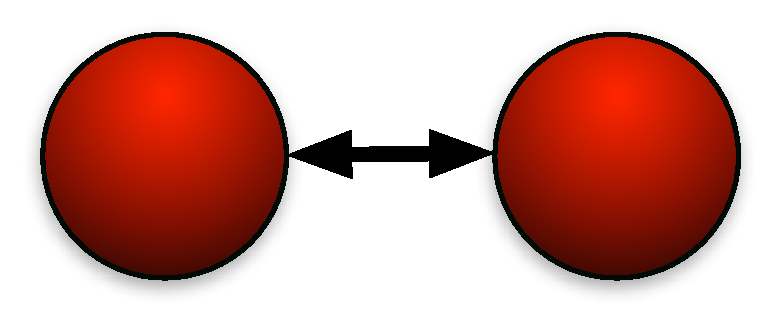
\includegraphics[scale=0.1]{../figures/sep_Craig.pdf}
			\caption{Collision Avoidance}
			\end{center}
			\end{figure}
		\end{column}
		\pause
		\begin{column}{4cm}
			\begin{figure}[htbp]
			\begin{center}
			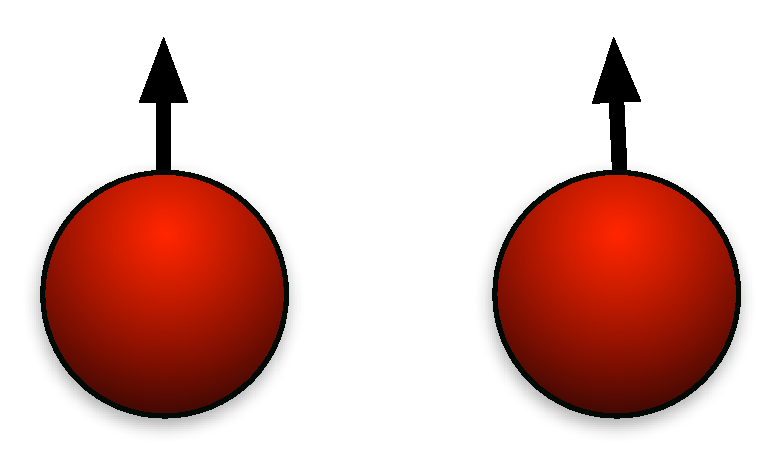
\includegraphics[scale=0.1]{../figures/align_Craig.pdf}
			\caption{Velocity Matching}
			\end{center}
			\end{figure}
		\end{column}
		\pause
		\begin{column}{4cm}
			\begin{figure}[htbp]
			\begin{center}
			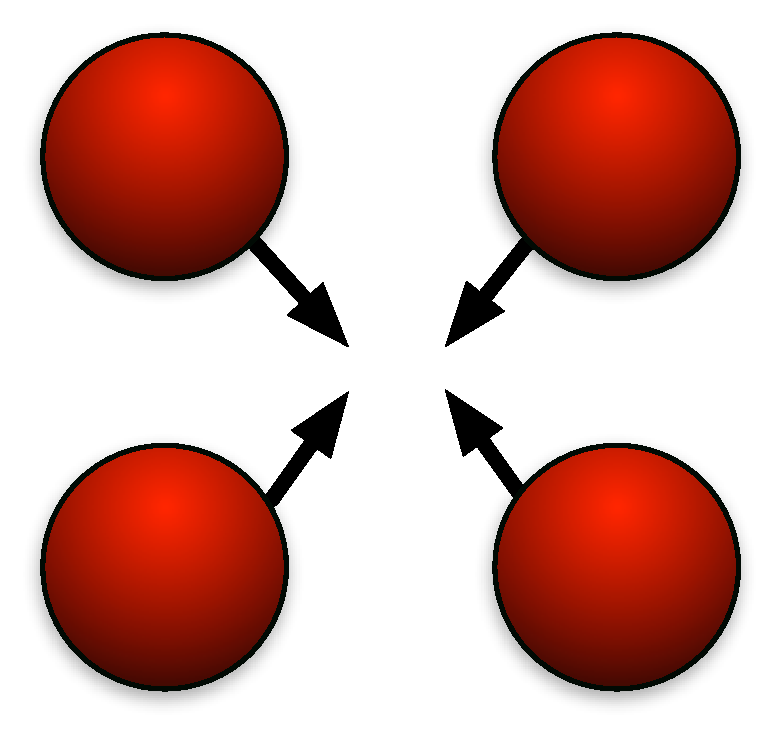
\includegraphics[scale=0.1]{../figures/coh_Craig.pdf}
			\caption{Flock Centering}
			\end{center}
			\end{figure}
		\end{column}
	\end{columns}		
\end{frame}


% other rules
\begin{frame}{Proceeding Work}
	\begin{itemize}
		\pause \item In 1999 Reynolds expanded the set of behaviors.
		\pause \item Some of the new behaviors were:
			\begin{itemize}
				\pause \item seek and pursuit
				\pause \item flee and evasion
				\pause \item obstacle avoidance
				\pause \item path following
				\pause \item leader following
				\pause \item among others...
			\end{itemize}
	\end{itemize}
\end{frame}
		
% applications
\begin{frame}{Applications}
	\begin{itemize}
		\pause \item Prey and predator simulations
		\pause \item Crowding simulations
		\pause \item Robotics
		\pause \item Unmanned air vehicles
		\pause \item Document clustering
	\end{itemize}
\end{frame}

% GPU computing
\begin{frame}{GPU Computing}
	\begin{itemize}
		\pause \item Graphics processing unit or GPU is a numeric computing engine used for massive computation.
		\pause \item \textit{GPU computing}, also know as \textit{GPGPU} is when we use GPUs for general computing.
		\pause \item \textit{GPU computing} is an heterogeneous system that uses GPUs and CPUs together to process a task.
		\pause \item GPUs have their own architecture therefore, they also have their own programming languages.
	\end{itemize}
\end{frame}

% flocking using the GPU
\begin{frame}{Flocking Using the GPU}
	\begin{itemize}
		\pause \item Flocking algorithms are parallelizable algorithms because the same operations are computed for all boids in the flock.
		\pause \item GPUs can be used to implement flocking algorithms and enhance the performance of the execution of the program.
	\end{itemize}
\end{frame}

%--------------------------------------------
% flocking algorithm
%--------------------------------------------
\section{Algorithm}

\begin{frame}{Flocking}
	\begin{itemize}
		\pause \item \textit{Flocking} is used to simulate social behavior between entities by following a simple set of rules.
		\pause \item These rules, also called \textit{steering behaviors} were introduced by Craig Reynolds and they are:
			\begin{itemize}
				\pause \item Separation
				\pause \item Alignment
				\pause \item Cohesion
			\end{itemize}
		\pause \item The steering behaviors are velocity vectors with direction and magnitude.
	\end{itemize}
\end{frame}

%--------------------------------------------
% 3 behaviors
%--------------------------------------------
\subsection{Three Main Steering Behaviors}

% separation
\begin{frame}{Separation}
	% equation: separation 
	\begin{equation}
	\label{separationEquation}
	Separation =\frac{1}{M} \sum_{n=1}^{M} \frac{p_i - p_n}{d(p_i,p_n)}
	\end{equation}
	
	% figure: separation
	\begin{figure}[htbp]
	\begin{center}
	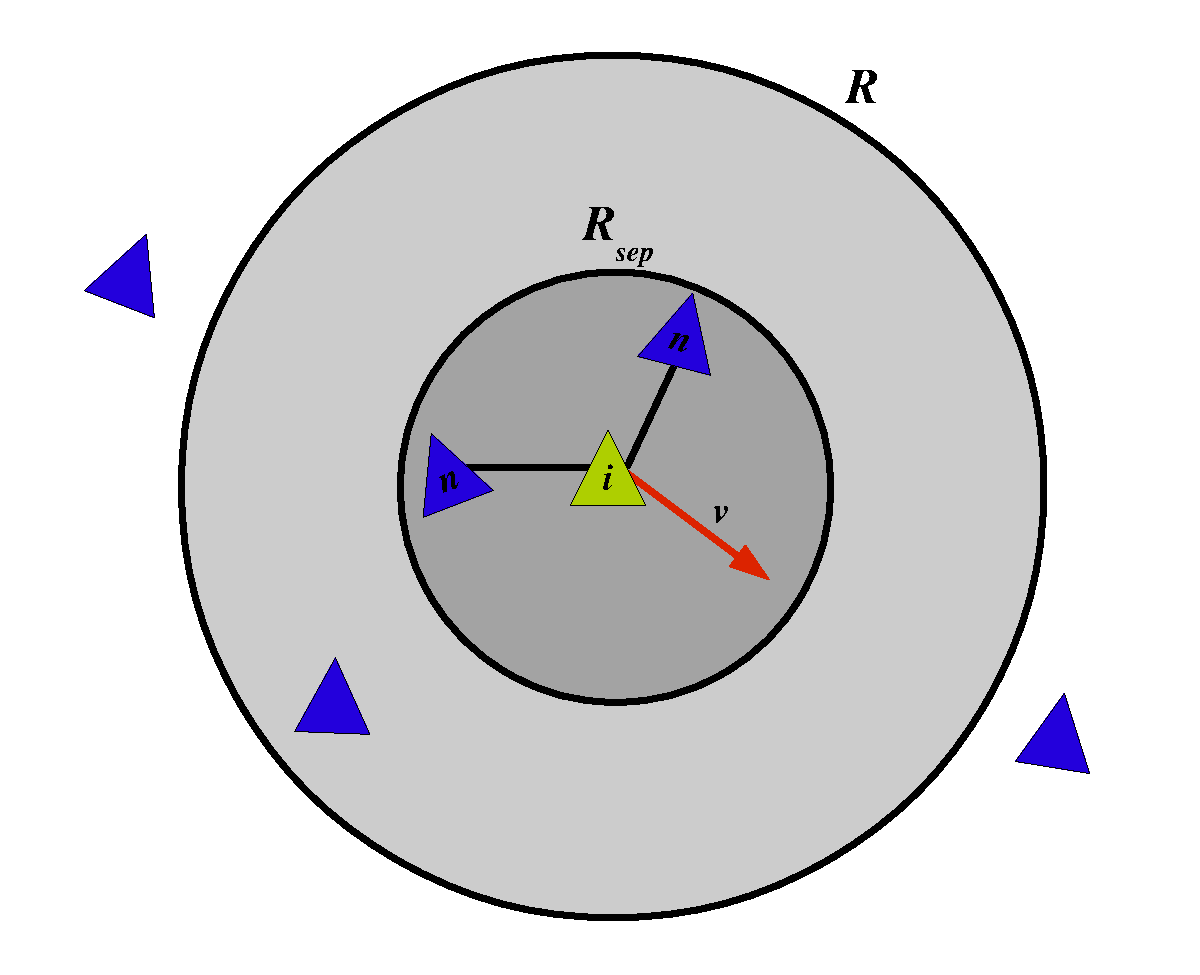
\includegraphics[scale=0.15]{../figures/separation.pdf}
	\caption{Separation steering behavior}
	\label{separation}
	\end{center}
	\end{figure}
\end{frame}

% alignment
\begin{frame}{Alignment}
	% equation: alignment
	\begin{equation}
	\label{alignmentEquation}
	Alignment = \left[  \frac{1}{N} \sum_{n=1}^{N} v_n \right ] - v_i
	\end{equation}
	
	% figure: alignment
	\begin{figure}[htbp]
	\begin{center}
	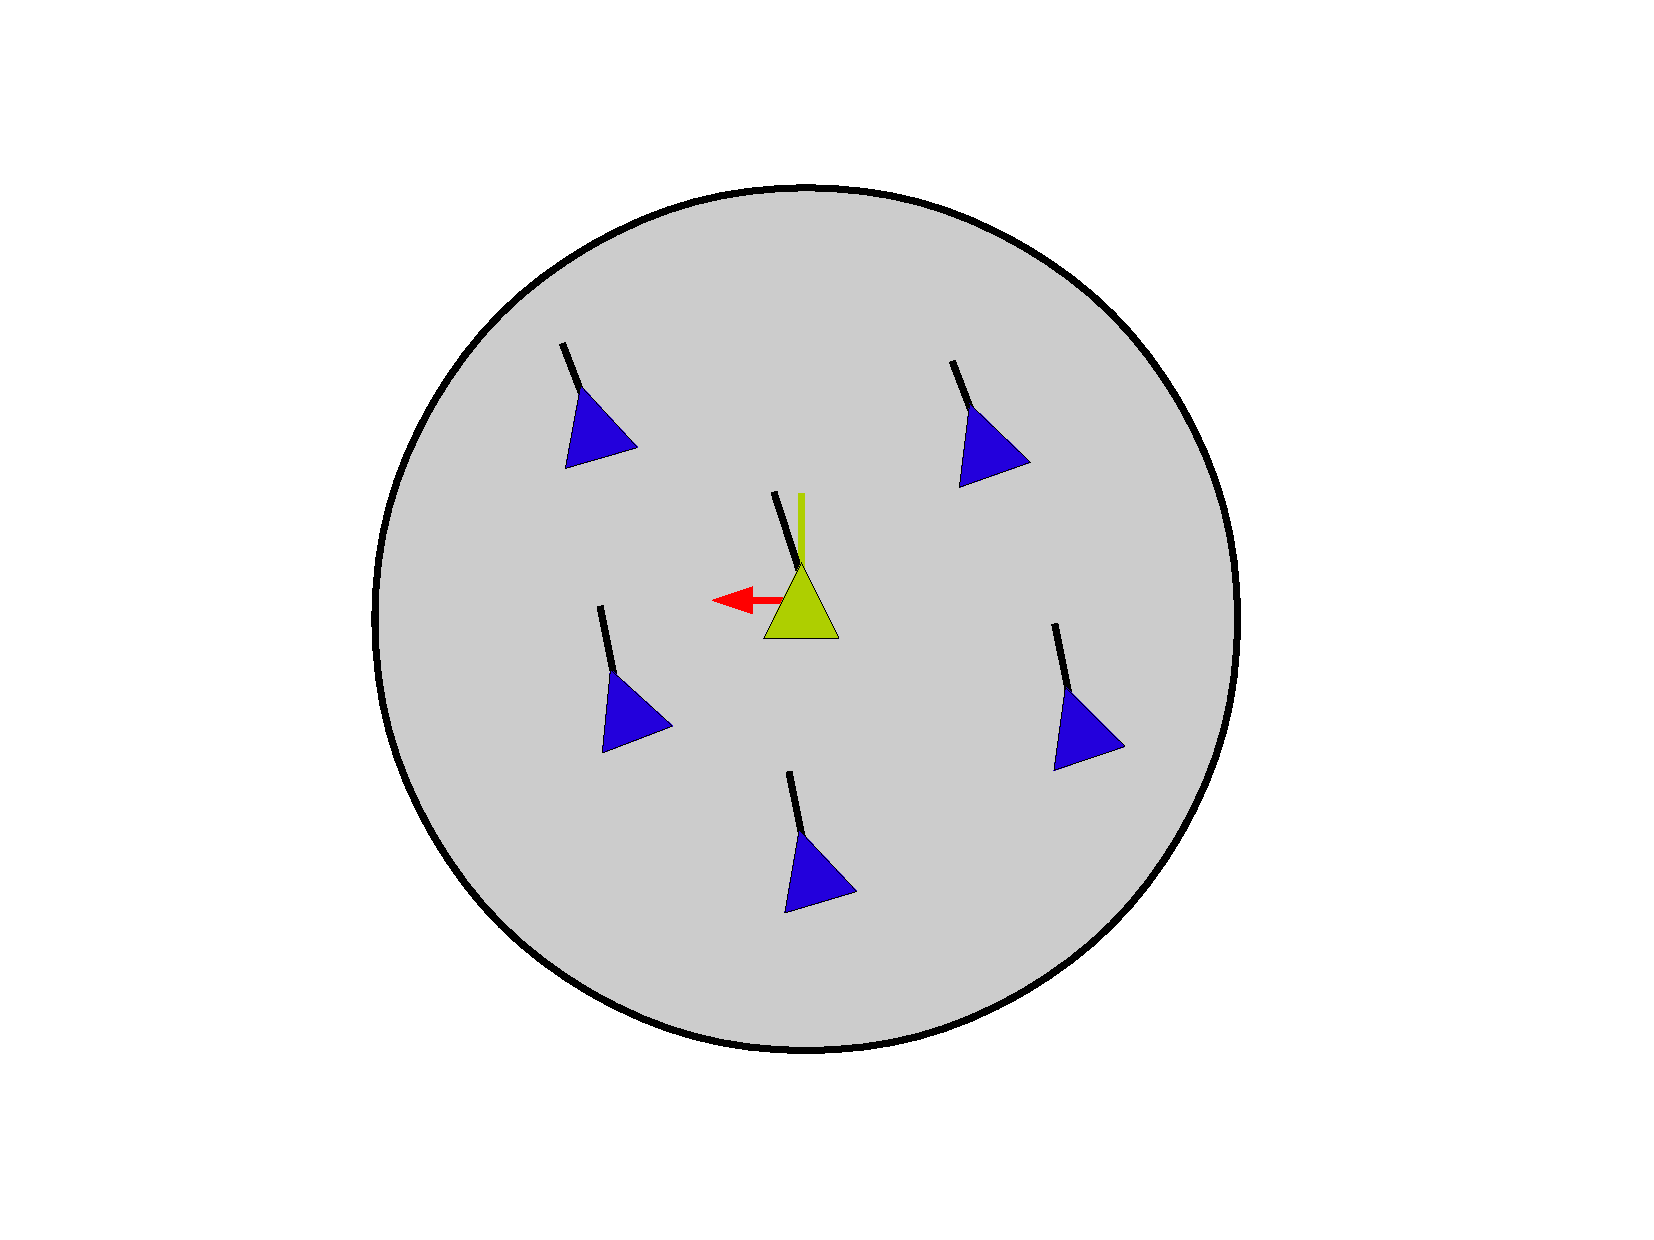
\includegraphics[scale=0.15]{../figures/alignment.pdf}
	\caption{Alignment steering behavior}
	\label{alignment}
	\end{center}
	\end{figure}
\end{frame}

% cohesion
\begin{frame}{Cohesion}
	% equation: cohesion
	\begin{equation}
	\label{cohesionEquation}
	Cohesion = \left[  \frac{1}{N} \sum_{n=1}^{N} p_n \right ] - p_i
	\end{equation}
	
	% figure: cohesion
	\begin{figure}[htbp]
	\begin{center}
	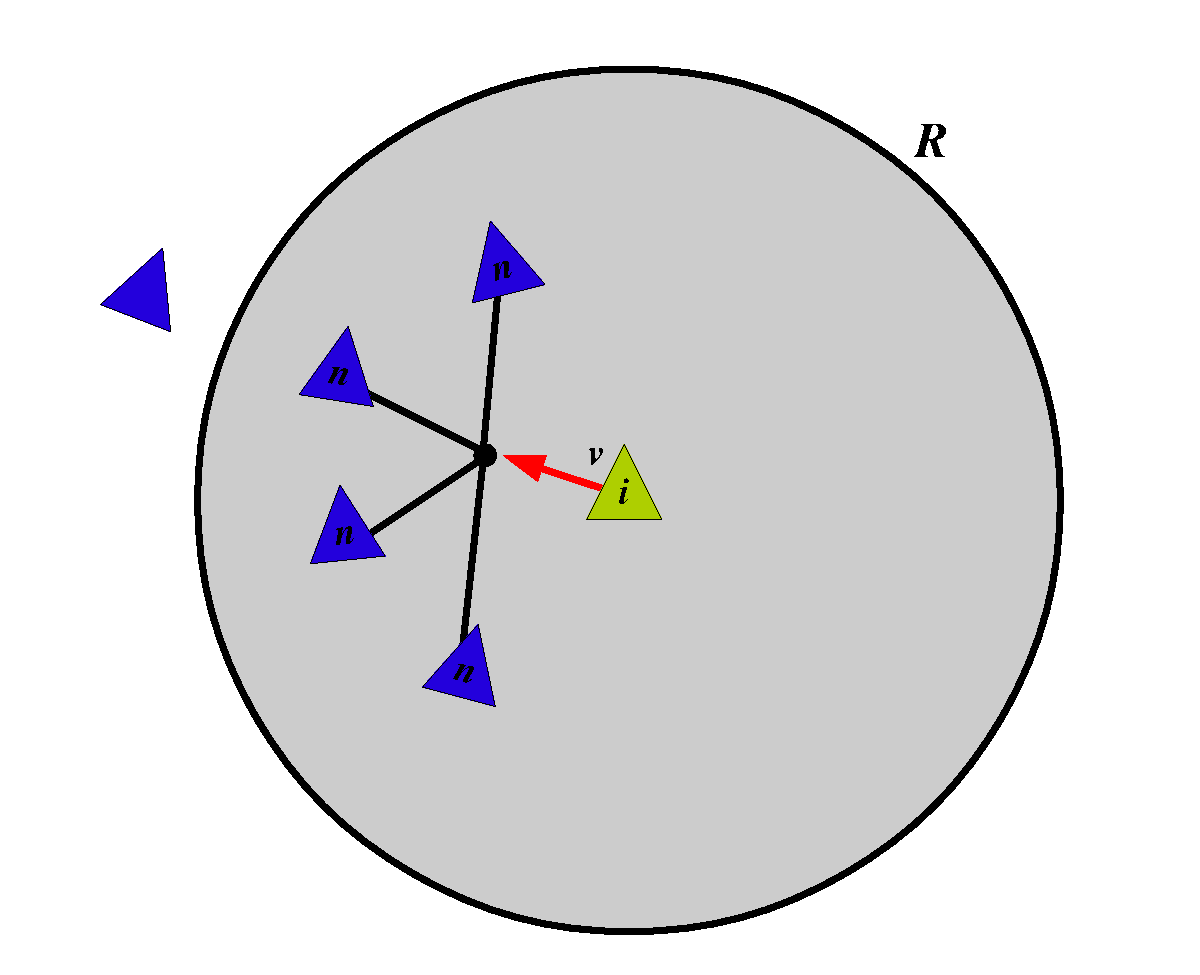
\includegraphics[scale=0.15]{../figures/cohesion.pdf}
	\caption{Cohesion steering behavior}
	\label{cohesion}
	\end{center}
	\end{figure}
\end{frame}

%--------------------------------------------
% other behaviors
%--------------------------------------------
\subsection{Other Steering Behaviors}

% goal and avoid
\begin{frame}{Goal and Avoid}

	% goal equation
	\begin{equation}
	\label{goalEquation}
	Goal = ((p_t - p_i) * max_{speed}) - v_i
	\end{equation}

	% avoid equation
	\begin{equation}
	\label{avoidEquation}
	Avoid = -((p_t - p_i) * max_{speed}) - v_i
	\end{equation}
	
	% figure: seek and flee
	\begin{figure}[htbp]
	\begin{center}
	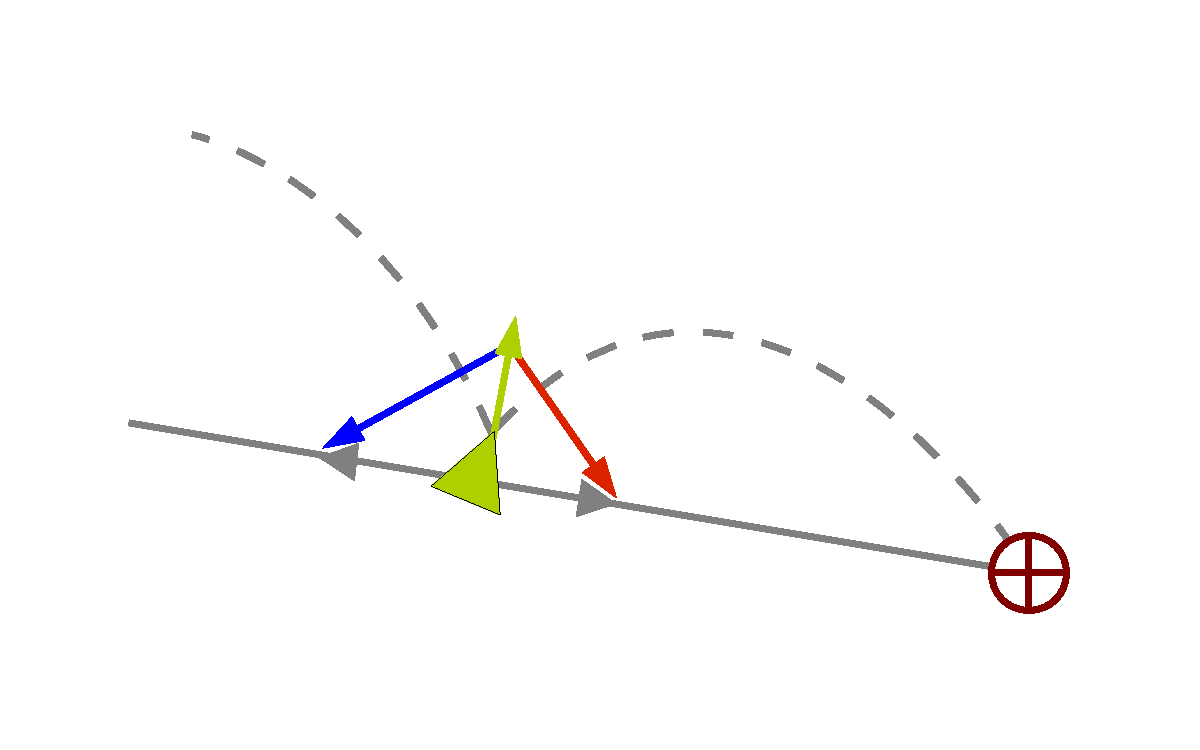
\includegraphics[scale=0.25]{../figures/seekANDflee.pdf}
	\caption{Goal and Avoid steering behavior}
	\label{seekANDflee}
	\end{center}
	\end{figure}
\end{frame}

% follow the leader
\begin{frame}{Follow the Leader}
	% figure: leader following
	\begin{figure}[htbp]
	\begin{center}
	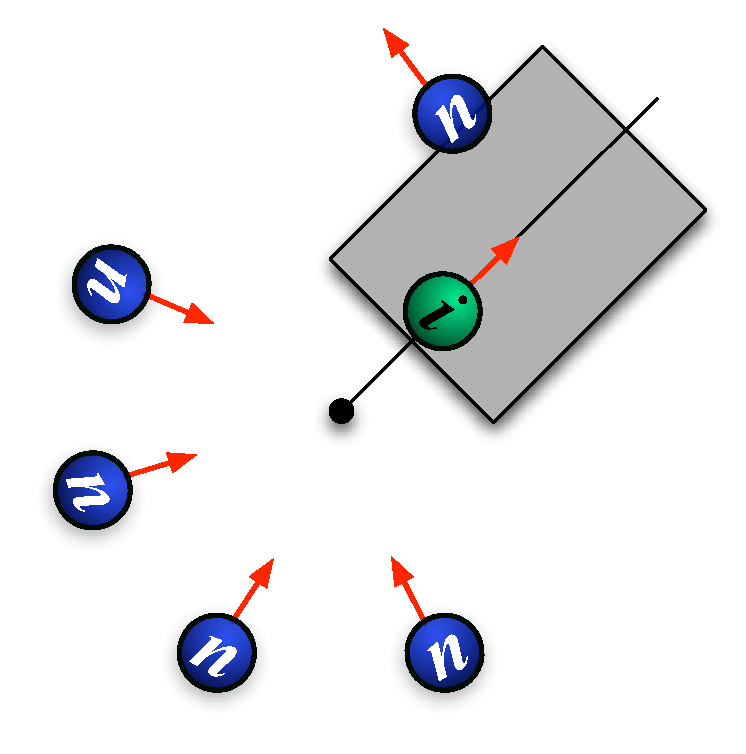
\includegraphics[scale=0.35]{../figures/leaderFollowing.pdf}
	\caption{Follow the leader steering behavior}
	\label{leadFollow}
	\end{center}
	\end{figure}
\end{frame}

%--------------------------------------------
% algorithm
%--------------------------------------------
\subsection{Flocking Algorithm}

% rules
\begin{frame}{Algorithm to compute the rules}
	\alert<1>{$for$ each neighbor $j$ of boid $i$ $do$}			\\
	\alert<2>{~~$if$ dist($pos_i$, $pos_j$) $<=$ searching radius $then$}	\\
	%\alert<3>{~~~~flockmates++}							\\
	\alert<4>{~~~~$if$ $w_{sep}$ $>$ 0 $then$}					\\
	\alert<4>{~~~~~~$if$ dist($pos_i$, $pos_j$) $<=$ minimum distance $then$}	\\
	\alert<4>{~~~~~~~~Compute the separation rule.} \\
	%\alert<4>{~~~~~~~~nearestFlockmates++}						\\
	%\alert<4>{~~~~~~~~s = $pos_i$ - $pos_j$} 					\\
	%\alert<4>{~~~~~~~~s /= dist($pos_i$, $pos_j$)} 						\\
	%\alert<4>{~~~~~~~~separation += s}							\\
	\alert<5>{~~~~$if$ $w_{align}$ $>$ 0 $then$}				\\
	\alert<5>{~~~~~~Compute the alignment rule.} \\
	%\alert<5>{~~~~~~alignment += $vel_j$}						\\
	\alert<6>{~~~~$if$ $w_{coh}$ $>$ 0 $then$}					\\
	\alert<6>{~~~~~~Compute the cohesion rule.} \\
	%\alert<6>{~~~~~~cohesion += $pos_j$}						\\
	\alert<7>{~~~~$if$ $w_{goal}$ $>$ 0 $then$}					\\
	\alert<7>{~~~~~~Compute the goal rule.} \\
	\alert<8>{~~~~$if$ $w_{avoid}$ $>$ 0 $then$}					\\
	\alert<8>{~~~~~~Compute the avoid rule.} \\
	\alert<9>{end $for$}
\end{frame}

% integration
\begin{frame}{Combine and Integrate}
 	%\alert<1>{$acc_{sep}$ = separation * $w_{sep}$}			\\
	%\alert<1>{$acc_{align}$ = alignment * $w_{align}$}		\\
	%\alert<1>{$acc_{coh}$ = cohesion * $w_{coh}$}			\\ 
 	\alert<1>{Multiply each rule by its weight to get the respective velocity.} 	\\
	%\alert<2>{$acc$ = $vel_i$ + $acc_{sep}$ + $acc_{align}$ + $acc_{coh}$} 	\\ 
	\alert<2>{Add the velocity of each rule and the current velocity.} 	\\
	\alert<3>{Constraint the velocity to a maximum speed.}			\\ 
	\alert<4>{Optional: Set any artificial velocity and add it to the velocity.}	\\ 
	%\alert<5>{$vel_i$ = $vel_{external}$ + $acc$}				\\ 
	%\alert<5>{Add the artificial velocity to the acceleration to get the \textit{new} velocity.} \\
	%\alert<6>{$pos_i$ +=  $dt $* $vel_i$}					\\
	\alert<5>{Multiply the \textit{new} velocity by the time step.}			\\
	\alert<6>{Add the velocity to the position to get the \textit{new} position.}	\\
\end{frame}

% each frame
\begin{frame}{Algorithm to update the simulation at each frame}
%\begin{tabbing}
	%\begin{block}{Algorithm to update the simulation at each frame}
		\alert<1>{Create a FLOCK particle system.}	\\
		\alert<2>{$for$ each frame $do$}			\\
		\alert<3>{~~Do the nearest neighbor search.}	\\
		\alert<4>{~~Compute the Rules.}				\\
		\alert<5>{~~Integrate over time.}				\\
		\alert<6>{~~Render the \textit{new} position.}	\\	
	%\end{block}
%\end{tabbing}
\end{frame}


%--------------------------------------------
% implementation
%--------------------------------------------
\section{Implementation}

%--------------------------------------------
% RTPS
%--------------------------------------------
\subsection{The RTPS Library}

% RTPS diagram
\begin{frame}{RTPS organization diagram}
	\begin{figure}[htbp]
	\begin{center}
	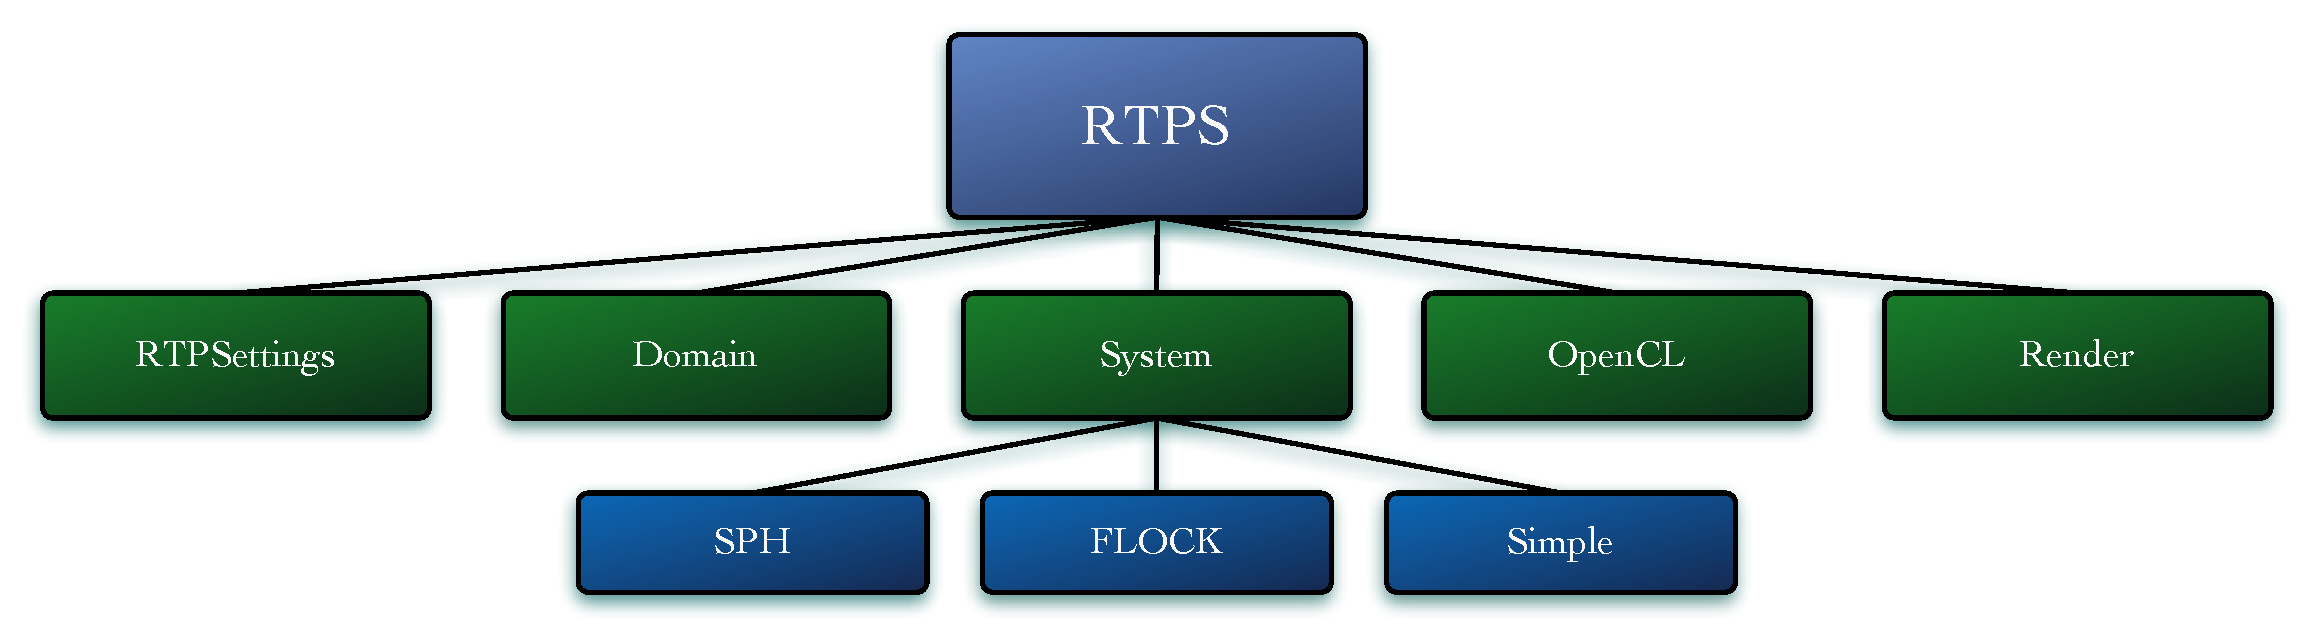
\includegraphics[scale=0.25]{../figures/RTPSdiagramMyrna.pdf}
	\caption{RTPS organization diagram}
	\end{center}
	\end{figure}
\end{frame}

% FLOCK diagram
\begin{frame}{FLOCK system organization diagram}
	\begin{figure}[htbp]
	\begin{center}
	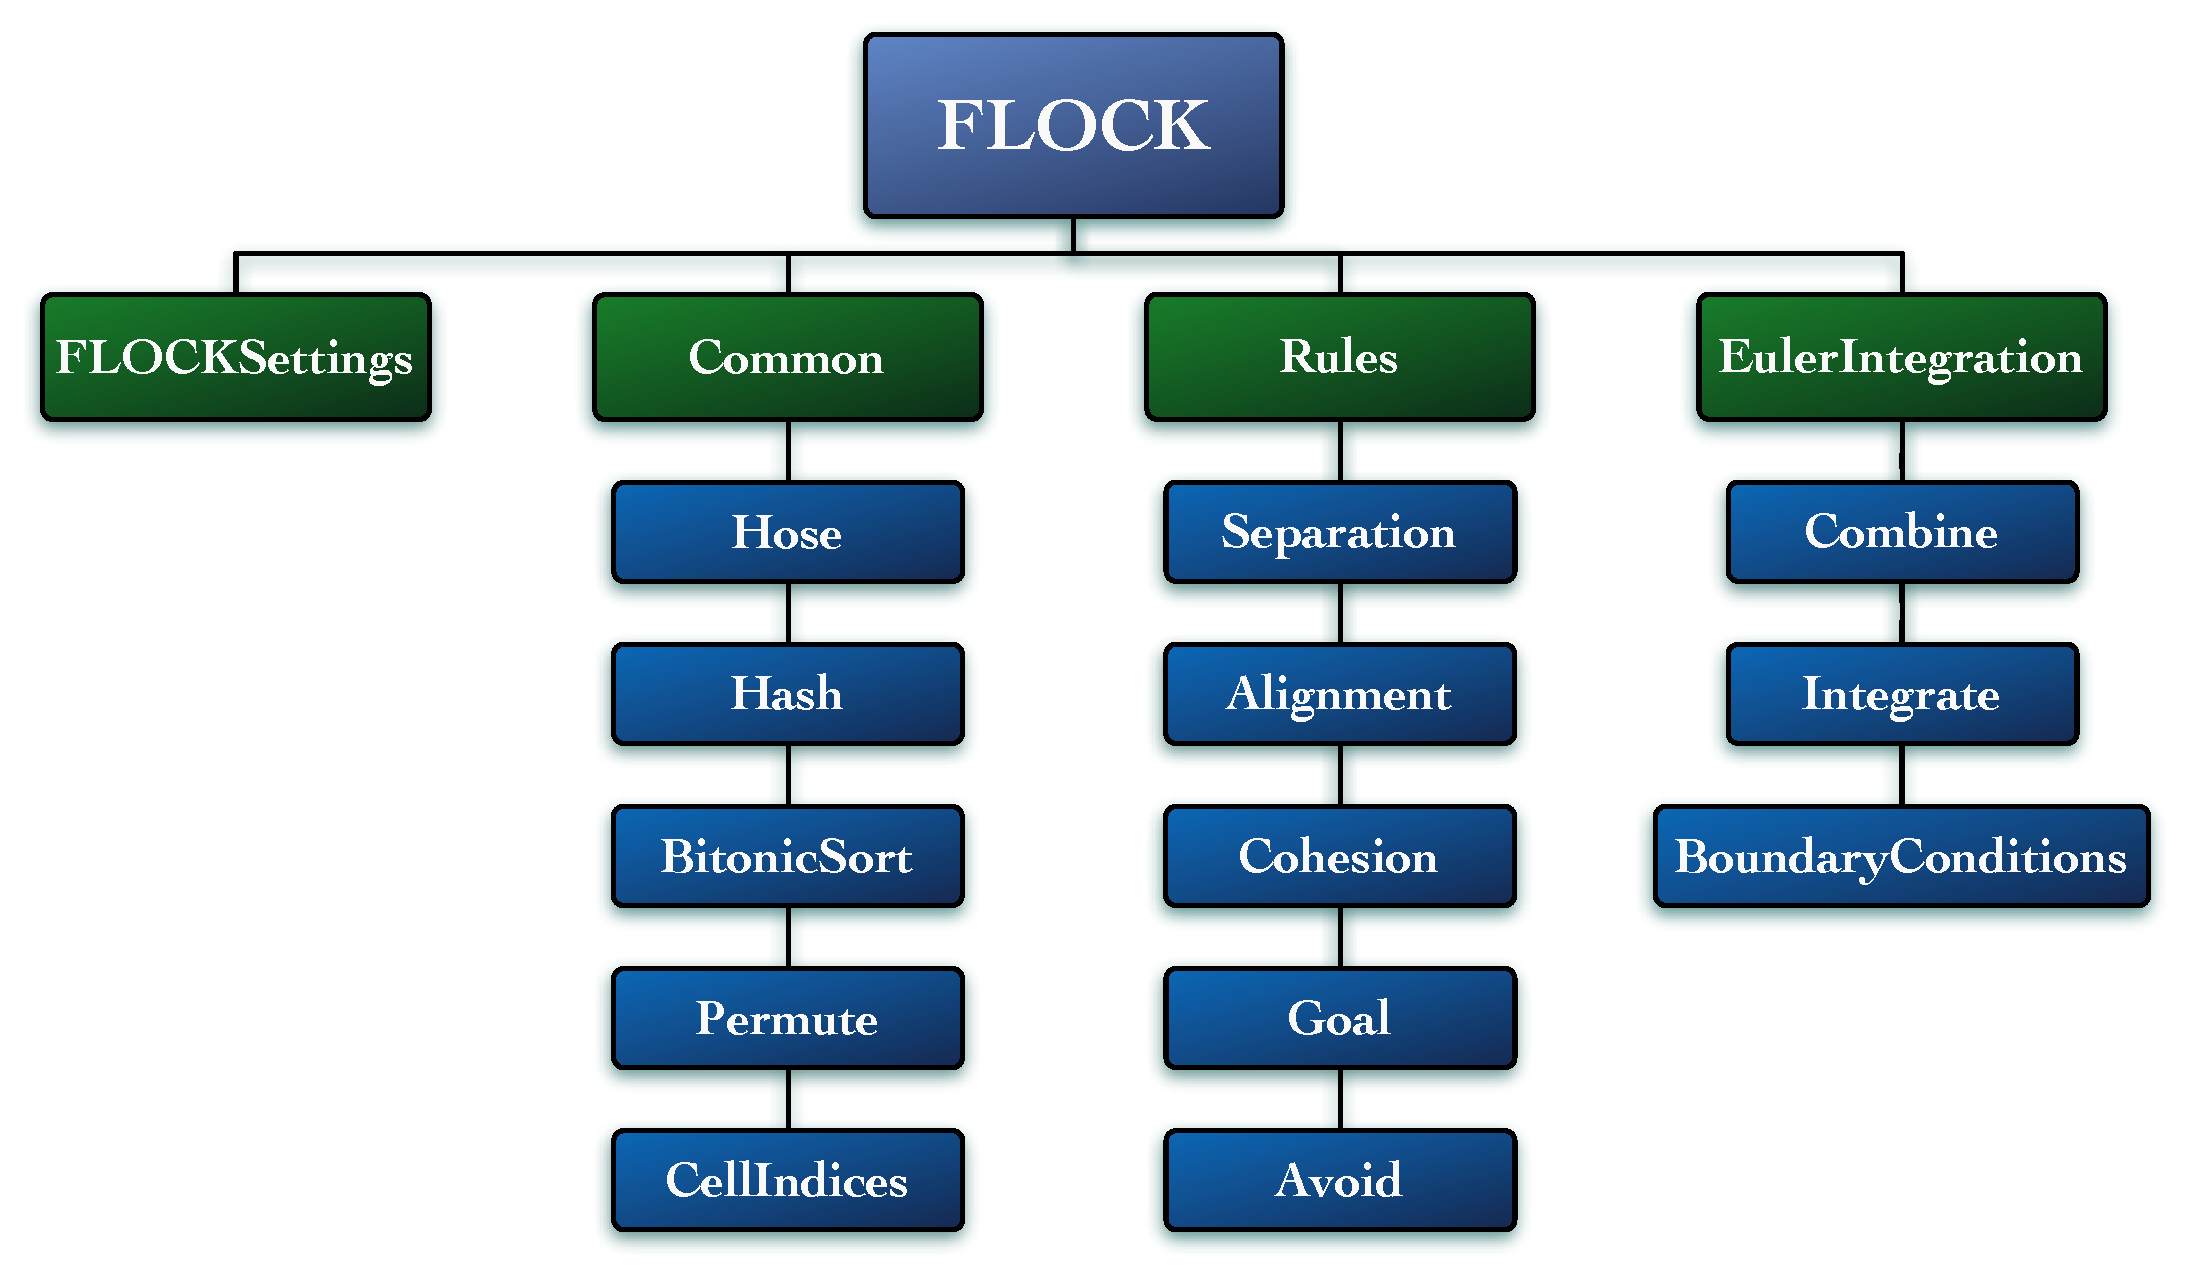
\includegraphics[scale=0.25]{../figures/FLOCKdiagramMyrna.pdf}
	\caption{FLOCK system organization diagram}
	\end{center}
	\end{figure}
\end{frame}

% FLOCK
%\begin{frame}{\texttt{FLOCK} class}
%	\begin{itemize}
%		\pause \item Main class of the FLOCK system
%		\pause \item Some of the objectives of this class are:
%			\begin{itemize}
%				\pause \item Create a FLOCK particle system.
%				\pause \item Call the respective functions to initialize the positions and velocities of the particles.
%				\pause \item Send the respective information to the GPU to do the calculations.
%				\pause \item Call the OpenCL kernel that computes the rules and the new positions.
%				 \pause \item Call the rendering method to render the particles on the screen.
%			\end{itemize}
%	\end{itemize}
%\end{frame}

% FLOCKSettings
%\begin{frame}{\texttt{FLOCKSettings} class}
%	\begin{itemize}
%		\pause \item Initialize the data structure that stores the settings of the FLOCK system.
%		\pause \item Update the values of the settings when the user changes them.
%	\end{itemize}
%\end{frame}

% Common
\begin{frame}{Common classes}
	\begin{itemize}
		\pause \item The common classes are:
			\begin{itemize}
				\pause \item Hash, BitonicSort, Permute, and CellIndices: classes that are in charge of the nearest neighbor search.
					\begin{itemize}
						\pause \item Hash: creates a hash value by overlaying the system into a uniform grid, and calculating an index value from the 3D cell index
						\pause \item BitonicSort: sorts the hash and index arrays by the hash values
						\pause \item Permute: permutes the arrays of positions, velocities and colors according to the sorted index array
						\pause \item CellIndices: updates two arrays that keep track of the first and last particle at each cell
					\end{itemize}
				\pause \item Hose: sprays particles into the system
			\end{itemize}
	\end{itemize}
\end{frame}

% FLOCK diagram
\begin{frame}{FLOCK system organization diagram}
	\begin{figure}[htbp]
	\begin{center}
	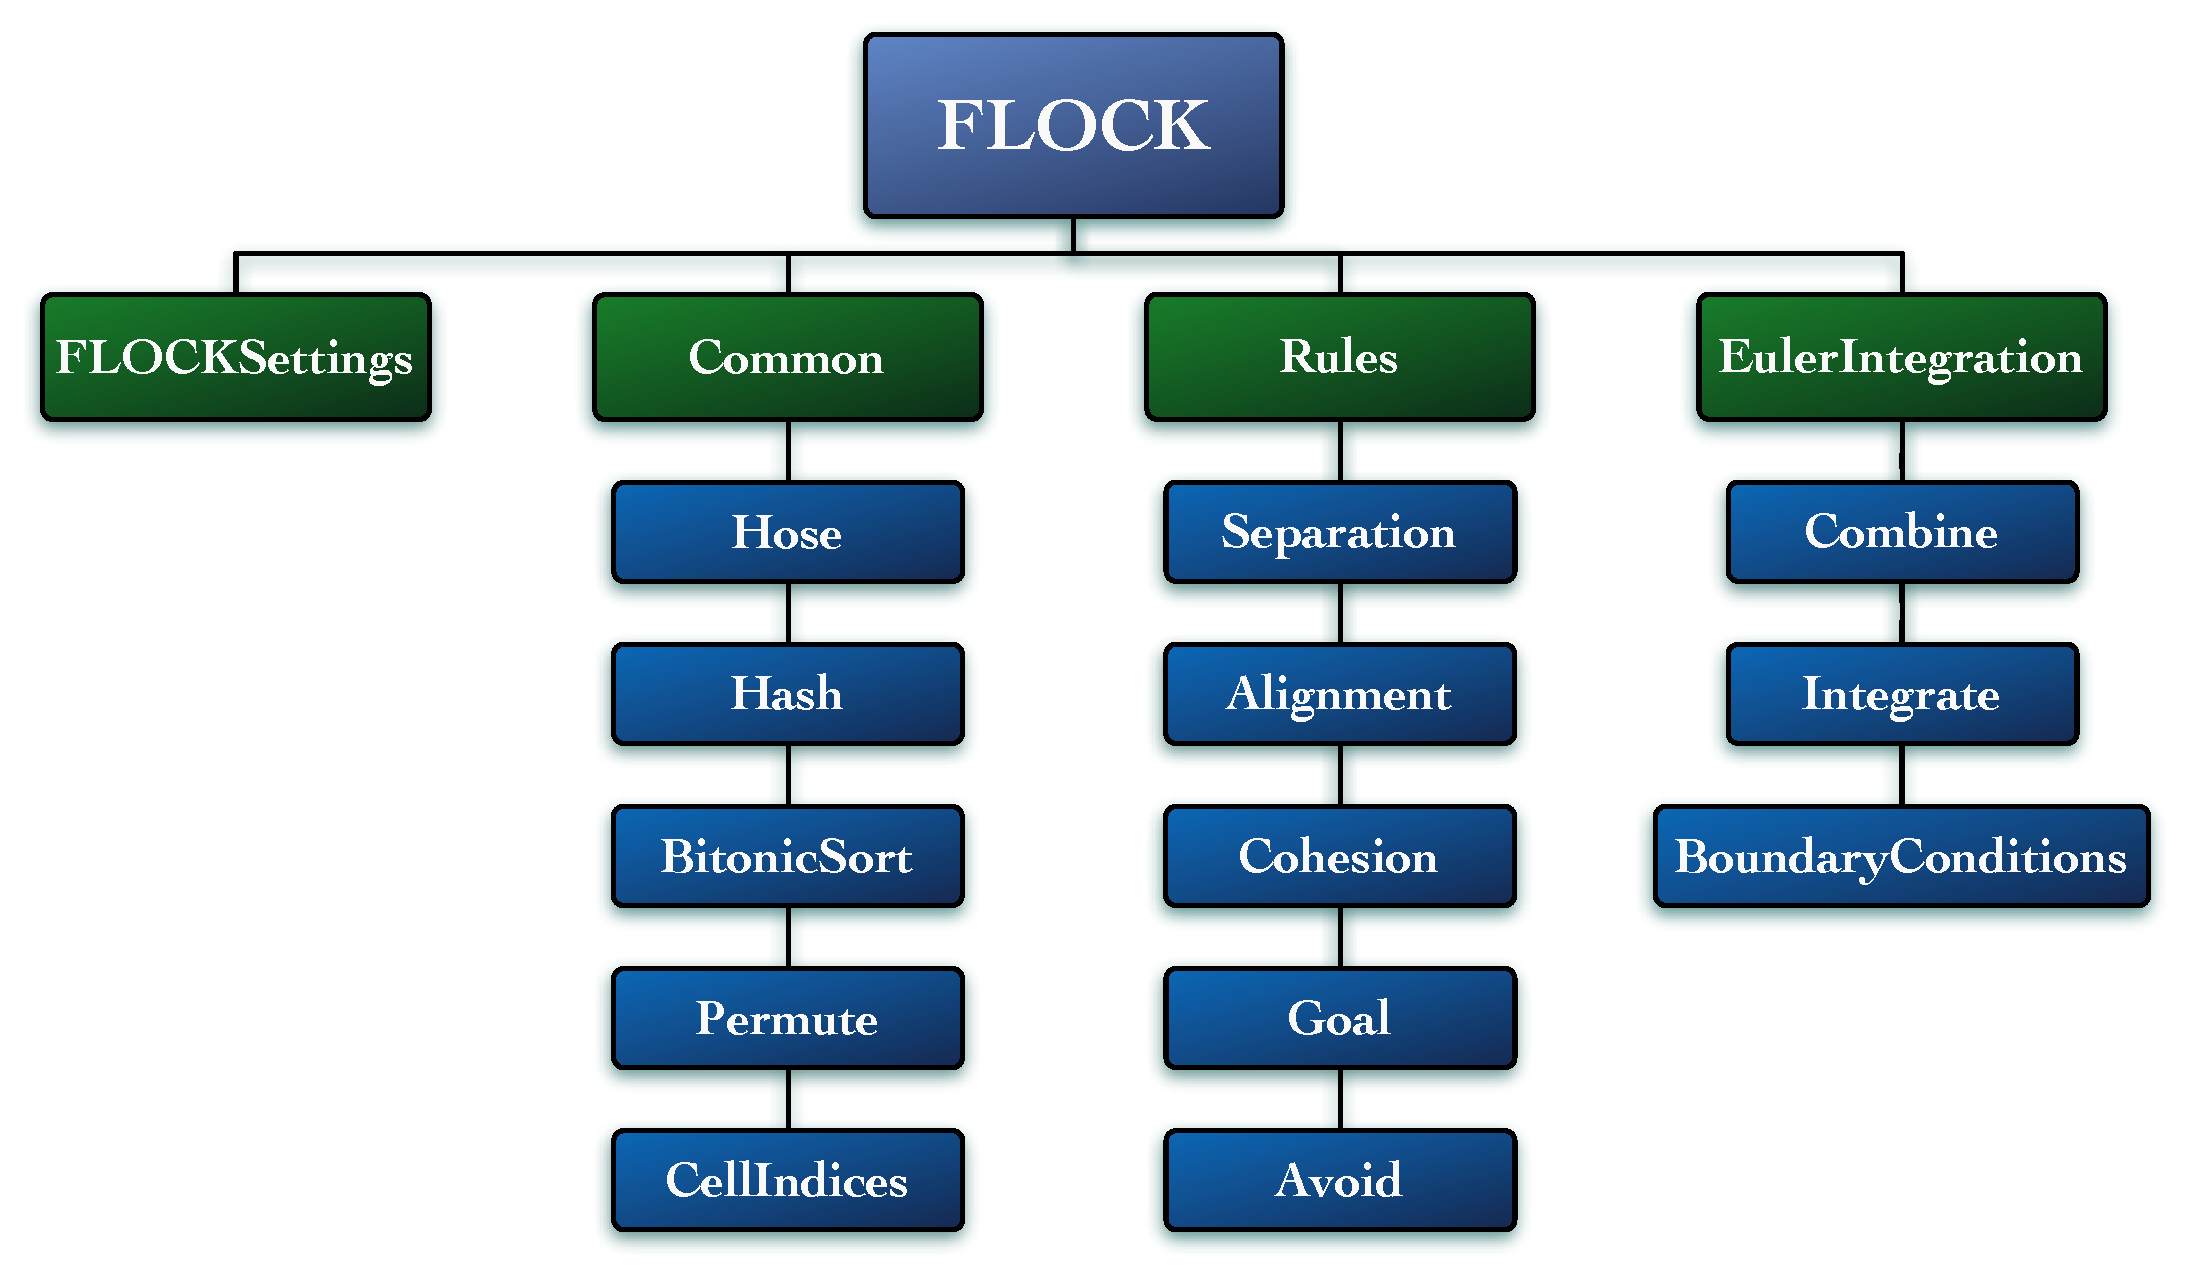
\includegraphics[scale=0.25]{../figures/FLOCKdiagramMyrna.pdf}
	\caption{FLOCK system organization diagram}
	\end{center}
	\end{figure}
\end{frame}

% Rules
%\begin{frame}{\texttt{Rules} class}
%	\begin{itemize}
%		\pause \item Create and initialize the OpenCL kernel that computes the rules.
%		\pause \item Set the arguments for the kernel.
%		\pause \item Launch the kernel.
%		\pause \item The kernel follows the previously discussed algorithm that computes the rules.
%	\end{itemize}
%\end{frame}

% EulerIntegration
%\begin{frame}{\texttt{EulerIntegration} class}
%	\begin{itemize}
%		\pause \item Has a similar structure than the \texttt{Rules} class.
%		\pause \item Its kernel follows the previously discussed algorithm that combine the rules and integrate over time to get the new position.
%		\pause \item Also, this kernel check the boundaries and apply periodic boundary conditions to the positions of the particles.
%	\end{itemize}
%\end{frame}

%--------------------------------------------
% blender
%--------------------------------------------
\subsection{The RTPS Modifier}

% Blender
\begin{frame}{Blender}
	\begin{itemize}
		\pause \item Blender is a free modeling/simulation software.
		\pause \item Blender has a built-in game engine.
		\pause \item Blender is open source.
		\pause \item Blender is cross-platform.
		\pause \item Blender supports simulations with real physics.
		\pause \item Blender has big support in the gaming industry and a large community helping on documentation.
		\pause \item Blender 2.57 was the release used in this project.
	\end{itemize}
\end{frame}

%--------------------------------------------
% BGE
%--------------------------------------------
\begin{frame}{The Blender Game Engine}
	\begin{itemize}
		\pause \item BGE is a very powerful tool.
		\pause \item Simple games can be created without the need for explicit programming.
		\pause \item After creating the 3D scene you can bring it to life by using the simple logic editor.
			% figure: logic editor 
			\pause
			\begin{figure}[htbp]
			\begin{center}
			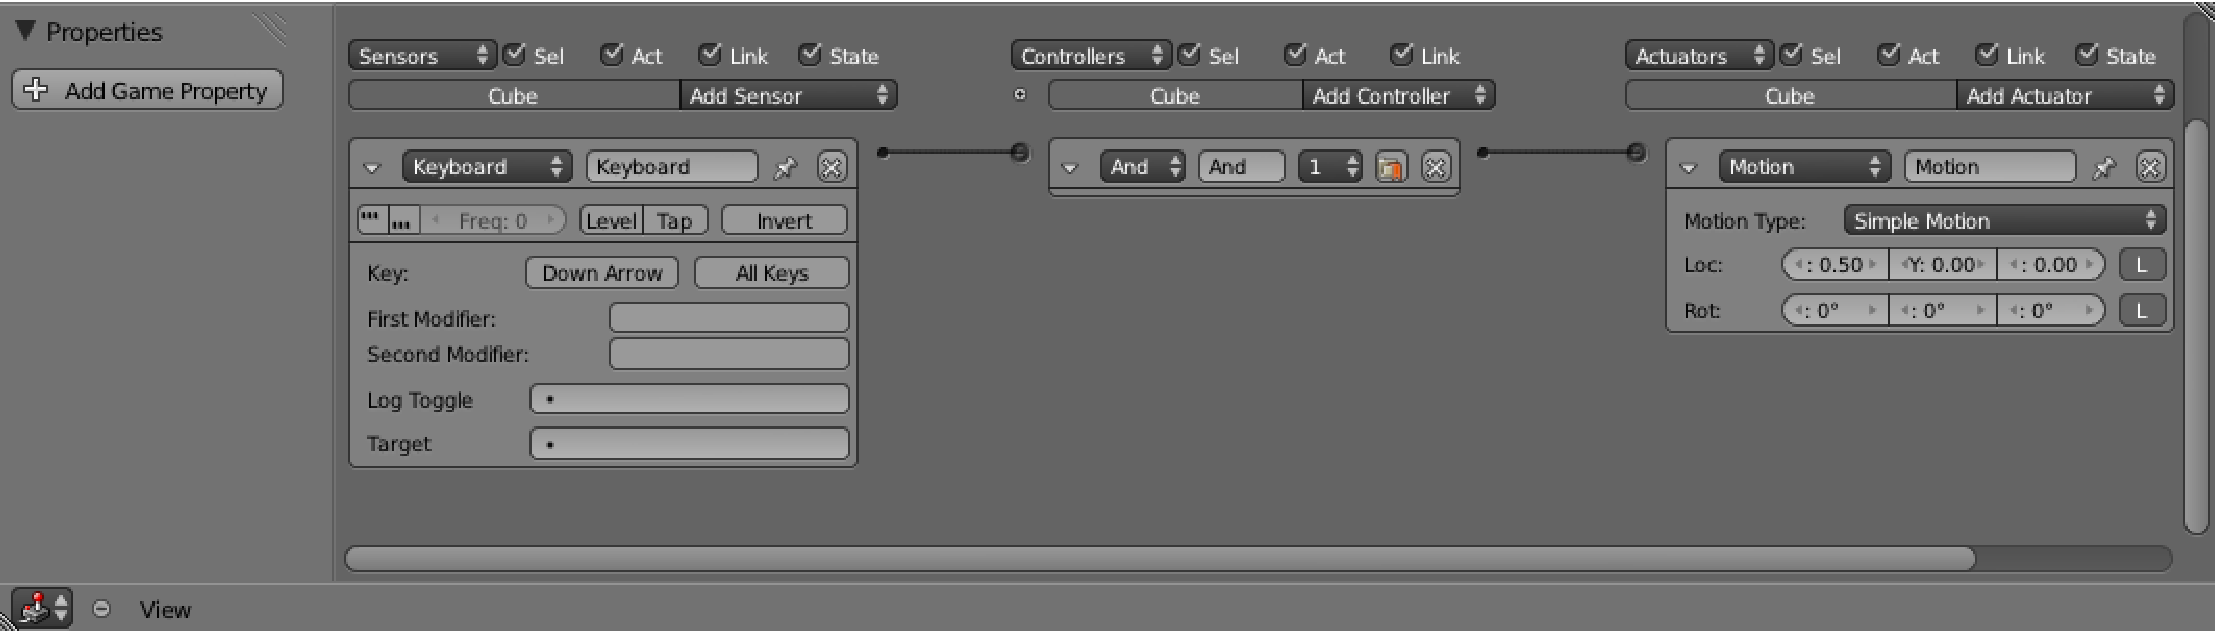
\includegraphics[scale=0.25]{../figures/logic.pdf}
			\caption{Blender Game Logic Editor}
			\label{logicEditor}
			\end{center}
			\end{figure}
	\end{itemize}
\end{frame}

% The Blender Game Engine
\begin{frame}{The Blender Game Engine}
	\begin{itemize}
		\pause \item The Blender Game Engine lacks of particles systems.
		\pause \item We would like to add this missing feature to it.
		\pause \item Boids particle systems are added to the Blender Game Engine in a modifier interface.
	\end{itemize}
\end{frame}

% The RTPS Modifier
\begin{frame}{The RTPS Modifier}
	\begin{figure}[htbp]
	\begin{center}
	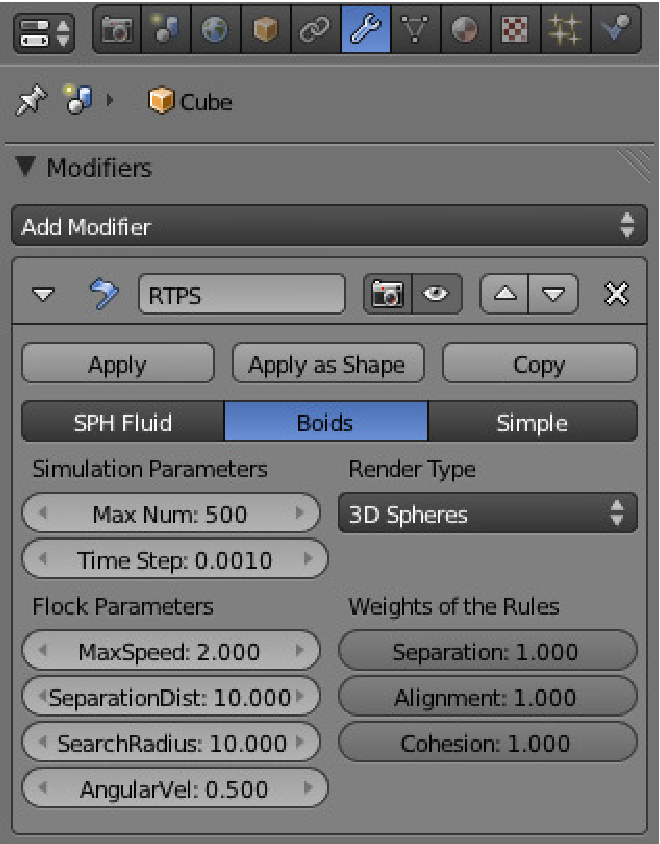
\includegraphics[scale=0.35]{../figures/modifier.pdf}
	\caption{The RTPS modifier in the Boids system}
	\end{center}
	\end{figure}
\end{frame}

\begin{frame}{Emitting particles to the system}
	\begin{table}[htdp]
	\caption{Properties available in the RTPS modifer}
	\begin{center}
	\begin{tabular}{|p{2cm}|p{6cm}|}
	\hline 
	\textbf{Property} & \textbf{Type and Description} \\\hline 
	\texttt{num} 	& \texttt{integer}: if num $>$ 0, num particles are going to be emitted every frame and num is set to 0	\\\hline 
	\texttt{hose}	& \texttt{boolean}: used to active the hose	\\\hline
	\texttt{speed}	& \texttt{float}: initial velocity of the particles that are going to be emitted from the hose	\\\hline
	\texttt{radius}	& \texttt{float}: width of the hose	\\
	\hline 
	\end{tabular}
	\end{center}
	\end{table}
\end{frame}


%--------------------------------------------
% results
%--------------------------------------------
\section{Results}

%--------------------------------------------
% timings
%--------------------------------------------
\subsection{Benchmarks}

% RTPS vs Blender
\begin{frame}{RTPS vs Blender}
	\begin{figure}[htbp]
	\begin{center}
	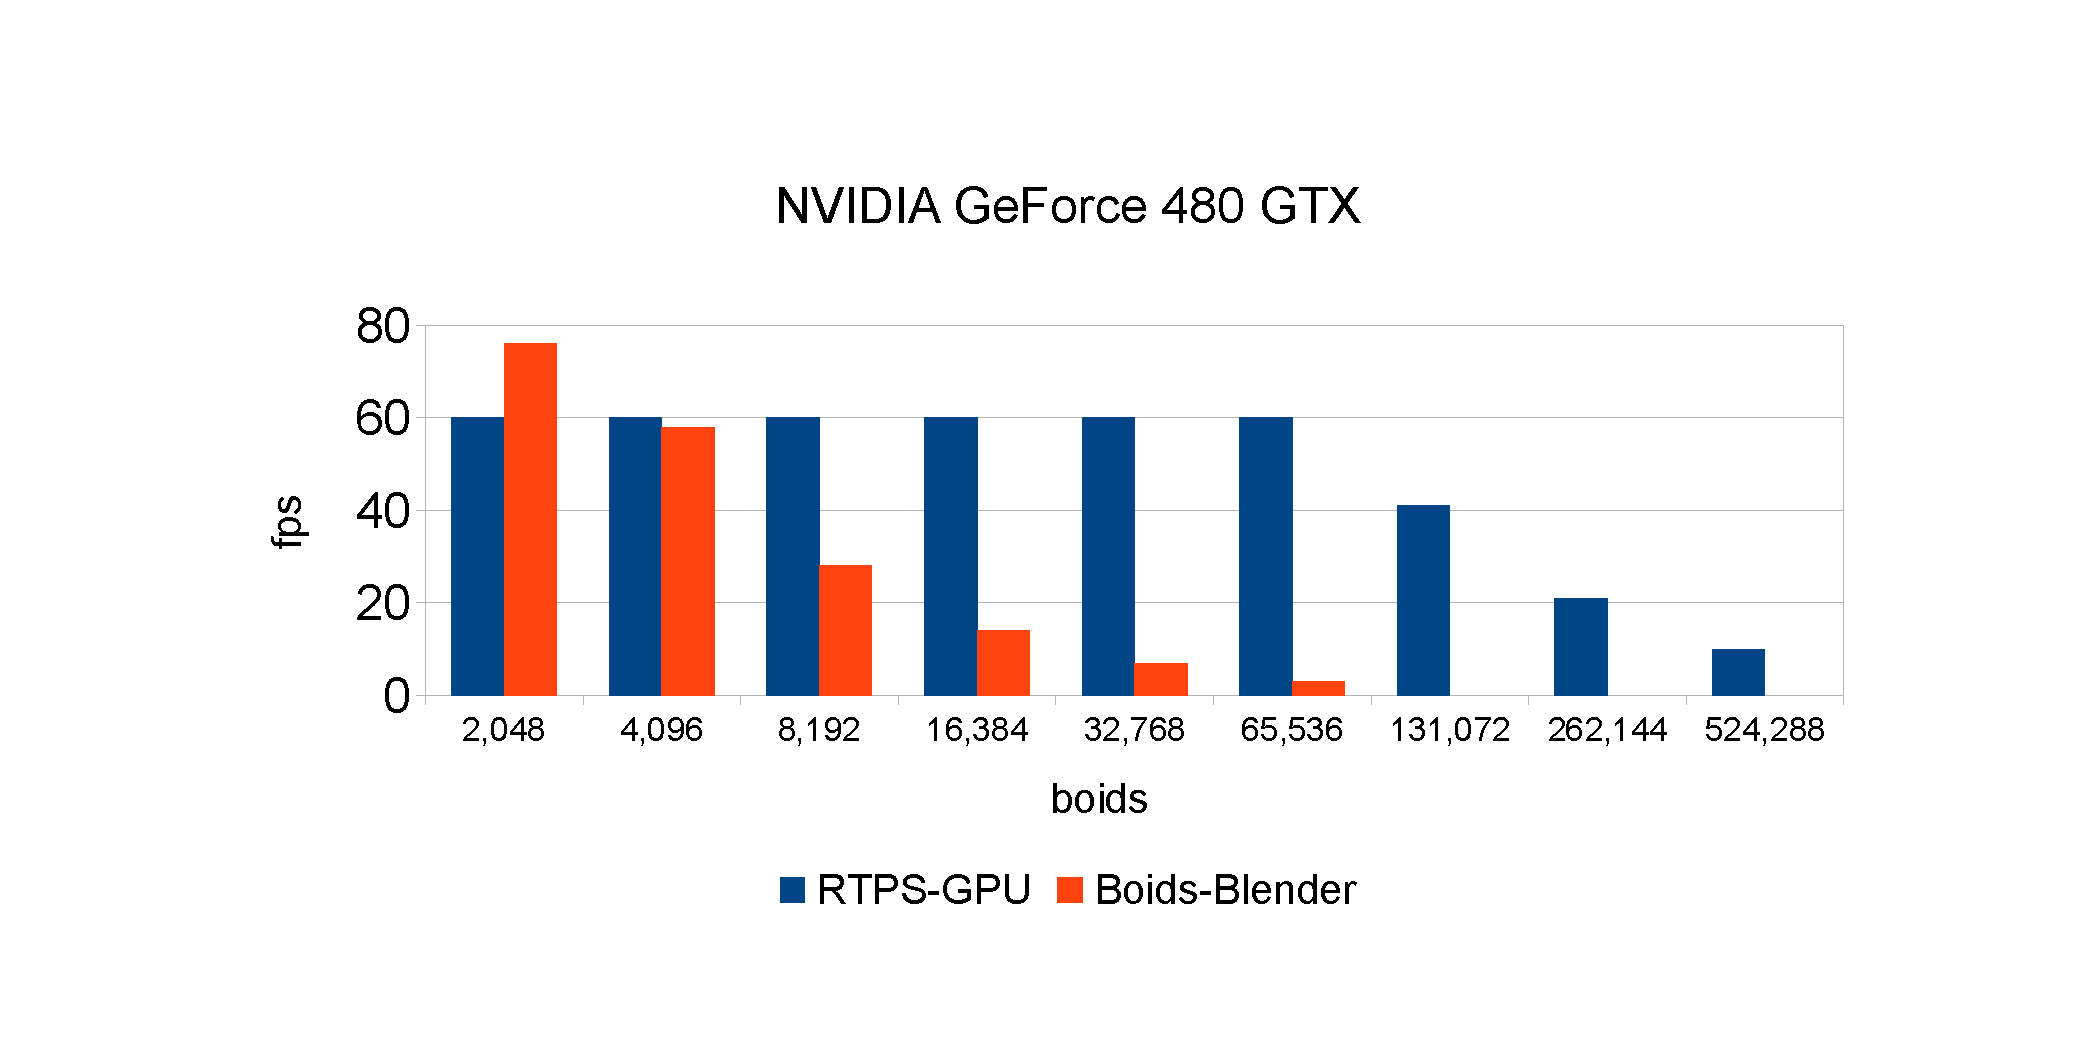
\includegraphics[scale=0.30]{../figures/benchmarks.pdf}
	\caption{Timings of RTPS modifier and Blender Boids system}
	\label{plot}
	\end{center}
	\end{figure}
\end{frame}

% RTPS Blender vs Blender
%\begin{frame}{RTPS Blender vs Blender}
%\textcolor{red}{*** MISSING ***}
%\end{frame}

% speedup
\begin{frame}{Speedup} 
	\begin{figure}[htbp]
	\begin{center}
	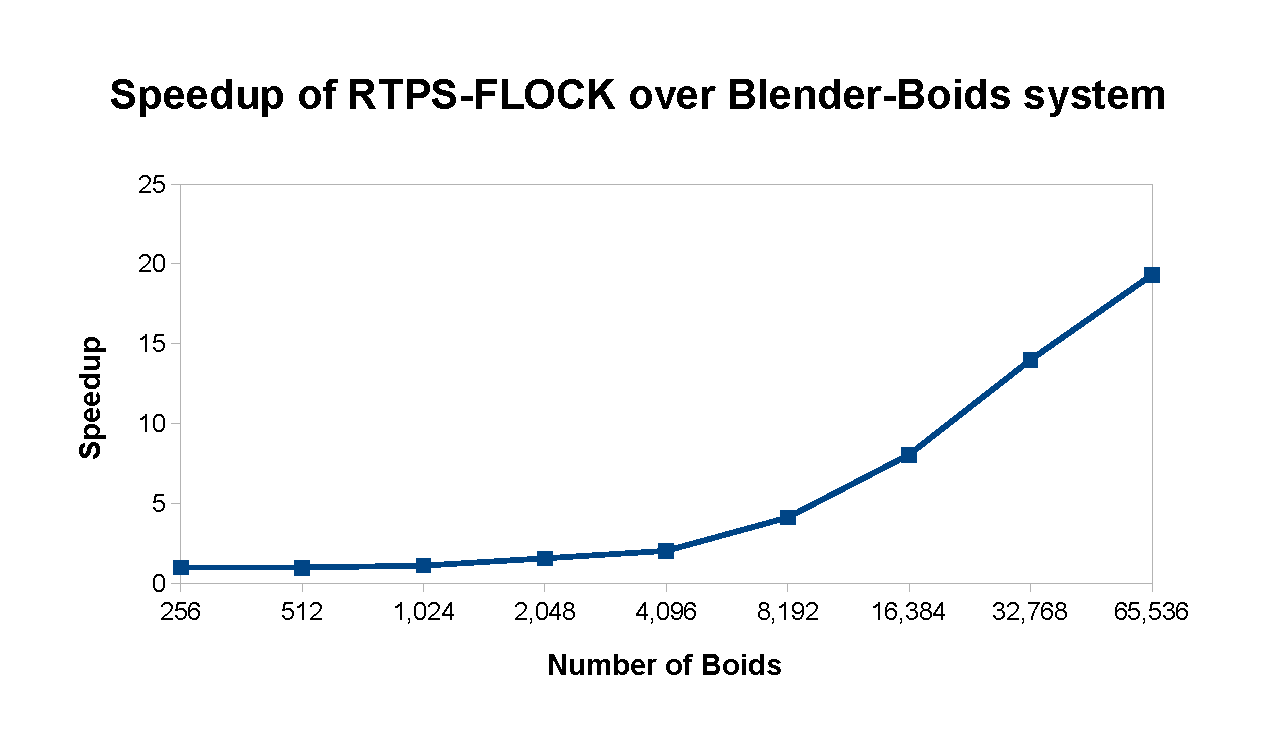
\includegraphics[scale=0.30]{../figures/speedup.pdf}
	\caption{Speedup of the FLOCK system of the RTPS library over the Blender Boids system}
	\label{speedup}
	\end{center}
	\end{figure}
\end{frame}

% RTPS kernels
\begin{frame}{RTPS kernels}
	\begin{figure}[htbp]
	\begin{center}
	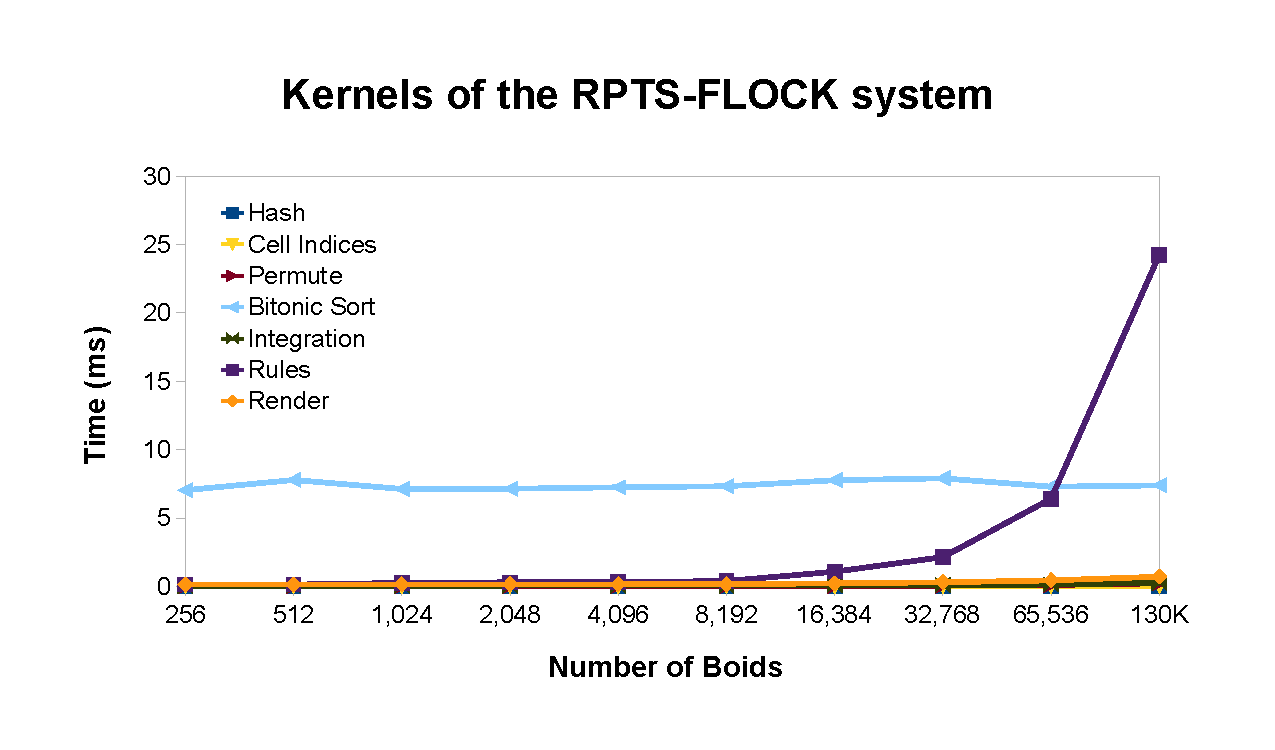
\includegraphics[scale=0.30]{../figures/kernelsPlot.pdf}
	\caption{Timings for the kernels executed by the FLOCK system of RTPS}
	\label{kernelBench}
	\end{center}
	\end{figure}
\end{frame}


%--------------------------------------------
% demos
%--------------------------------------------
\subsection{Demos}

% Symmetry
\begin{frame}{Symmetry Demo}
	\begin{figure}[htbp]
	\begin{center}
	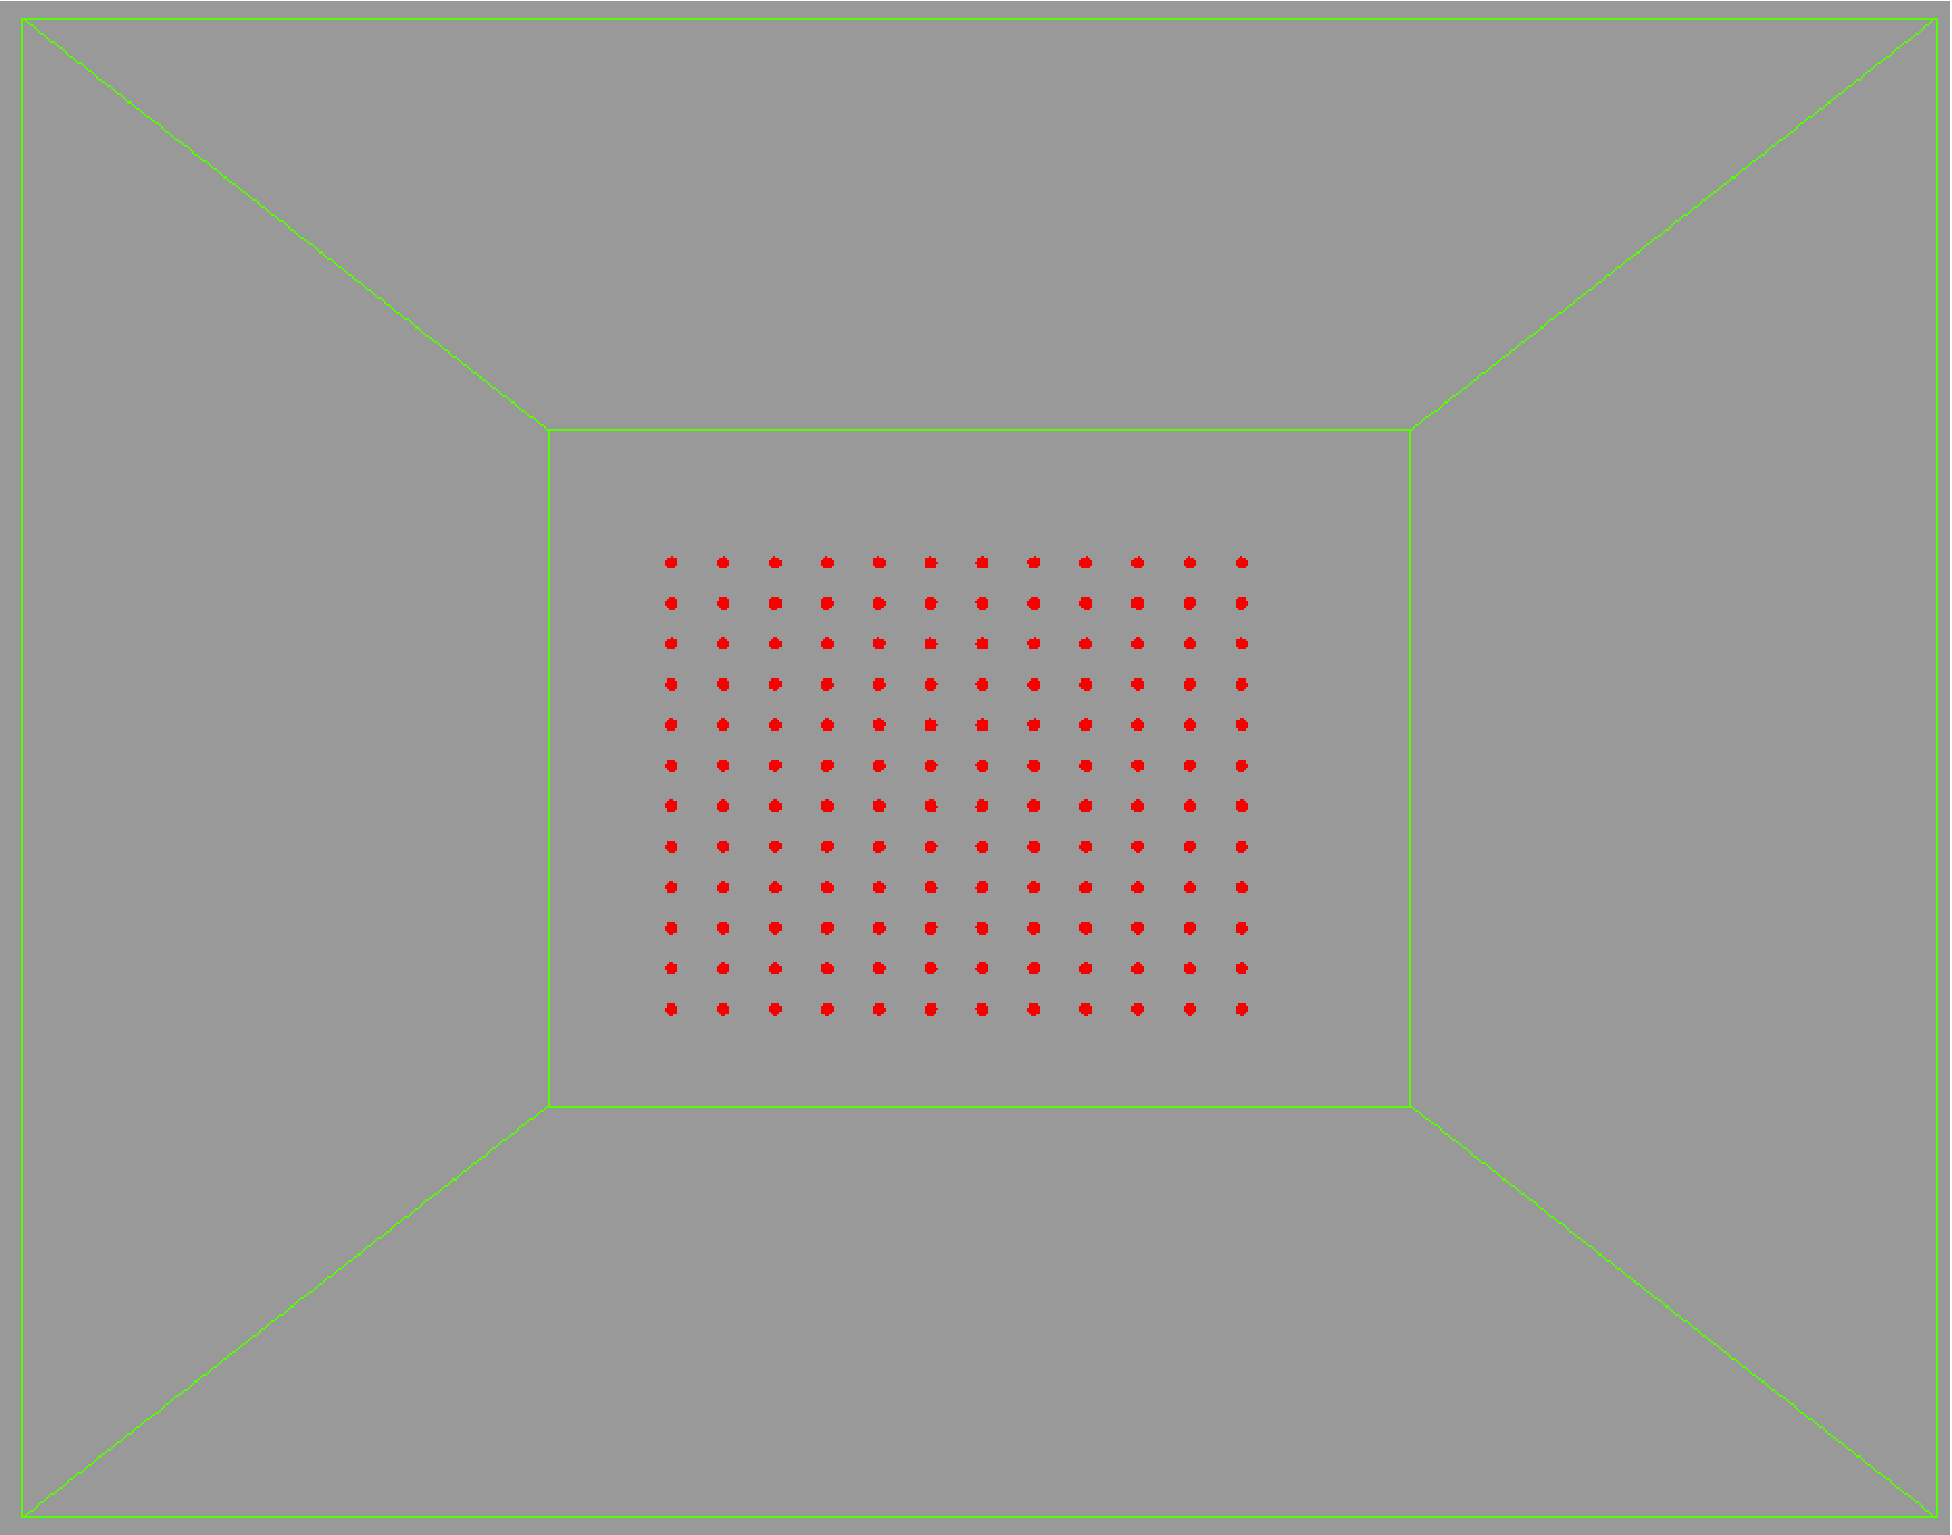
\includegraphics[scale=0.35]{../figures/align.pdf}
	\caption{Initial state of the boids}
	\label{alignRule}
	\end{center}
	\end{figure}
\end{frame}

\begin{frame}{Symmetry Demo}
	\begin{figure}[htbp]
	\begin{center}$
	\begin{array}{cc}
	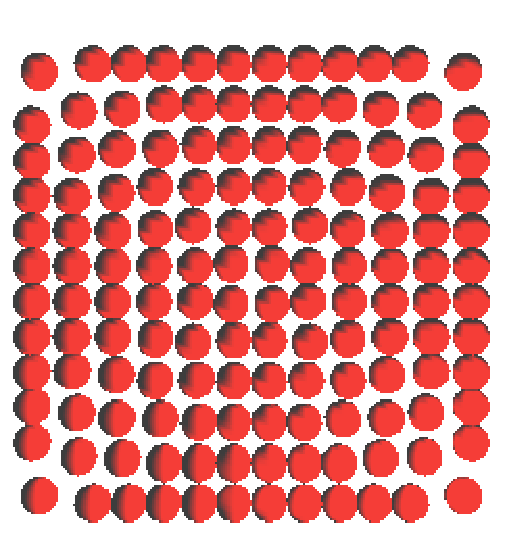
\includegraphics[scale= 0.35]{../figures/sep1.pdf} &
	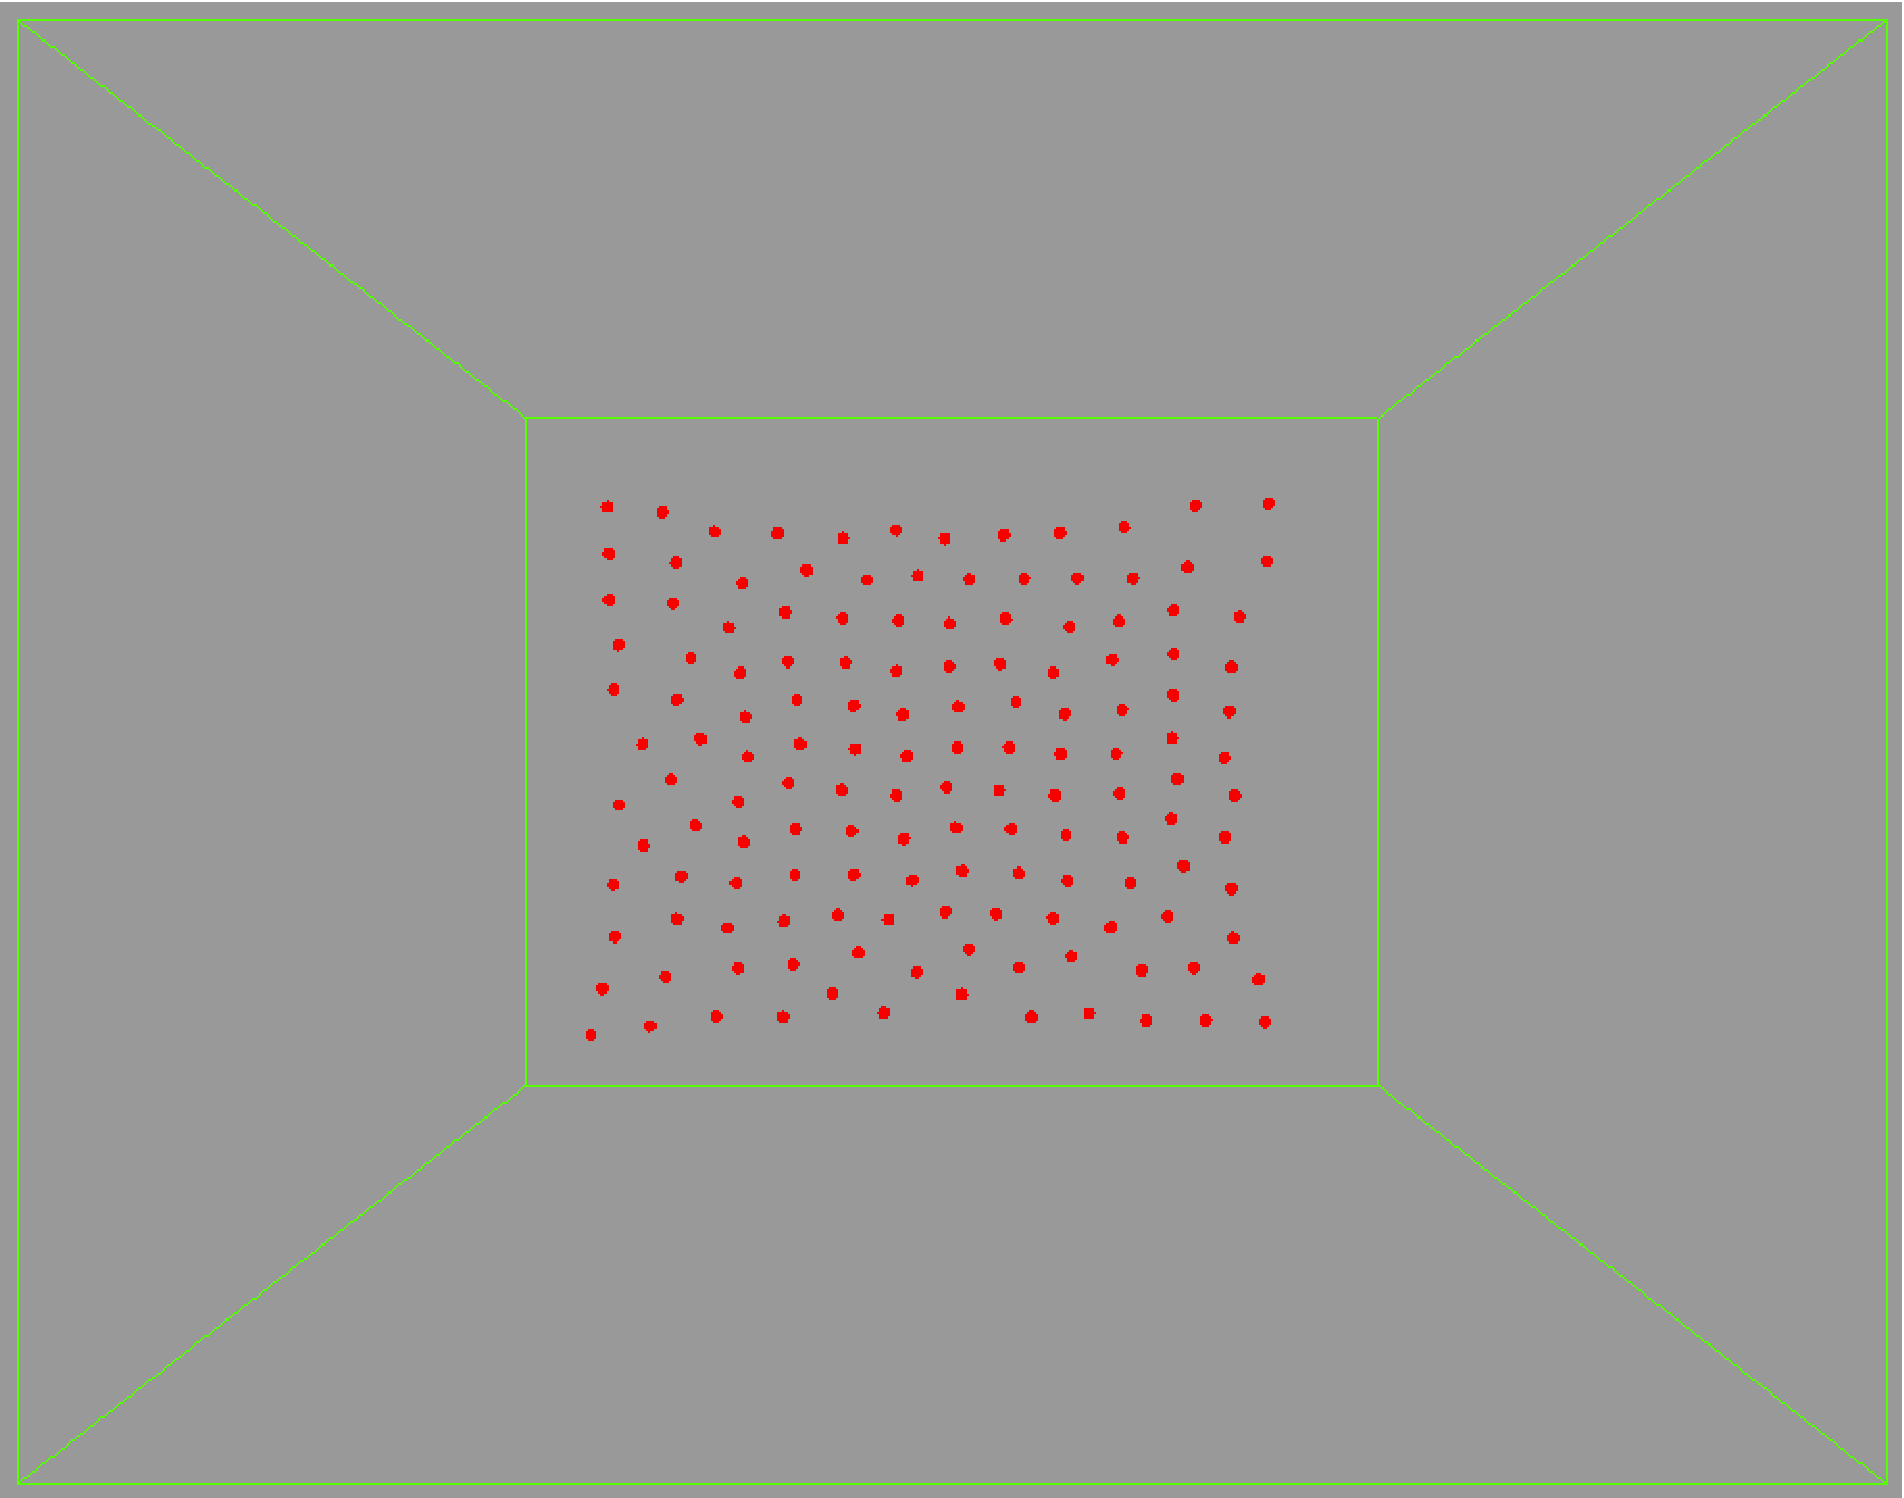
\includegraphics[scale= 0.35]{../figures/sep2.pdf}
	\end{array}$
	\end{center}
	\caption{Screenshots of the separation rule}
	\label{sepRule}
	\end{figure}
\end{frame}

\begin{frame}{Symmetry Demo}
	\begin{figure}[htbp]
	\begin{center}
	\begin{tabular}{cc}
	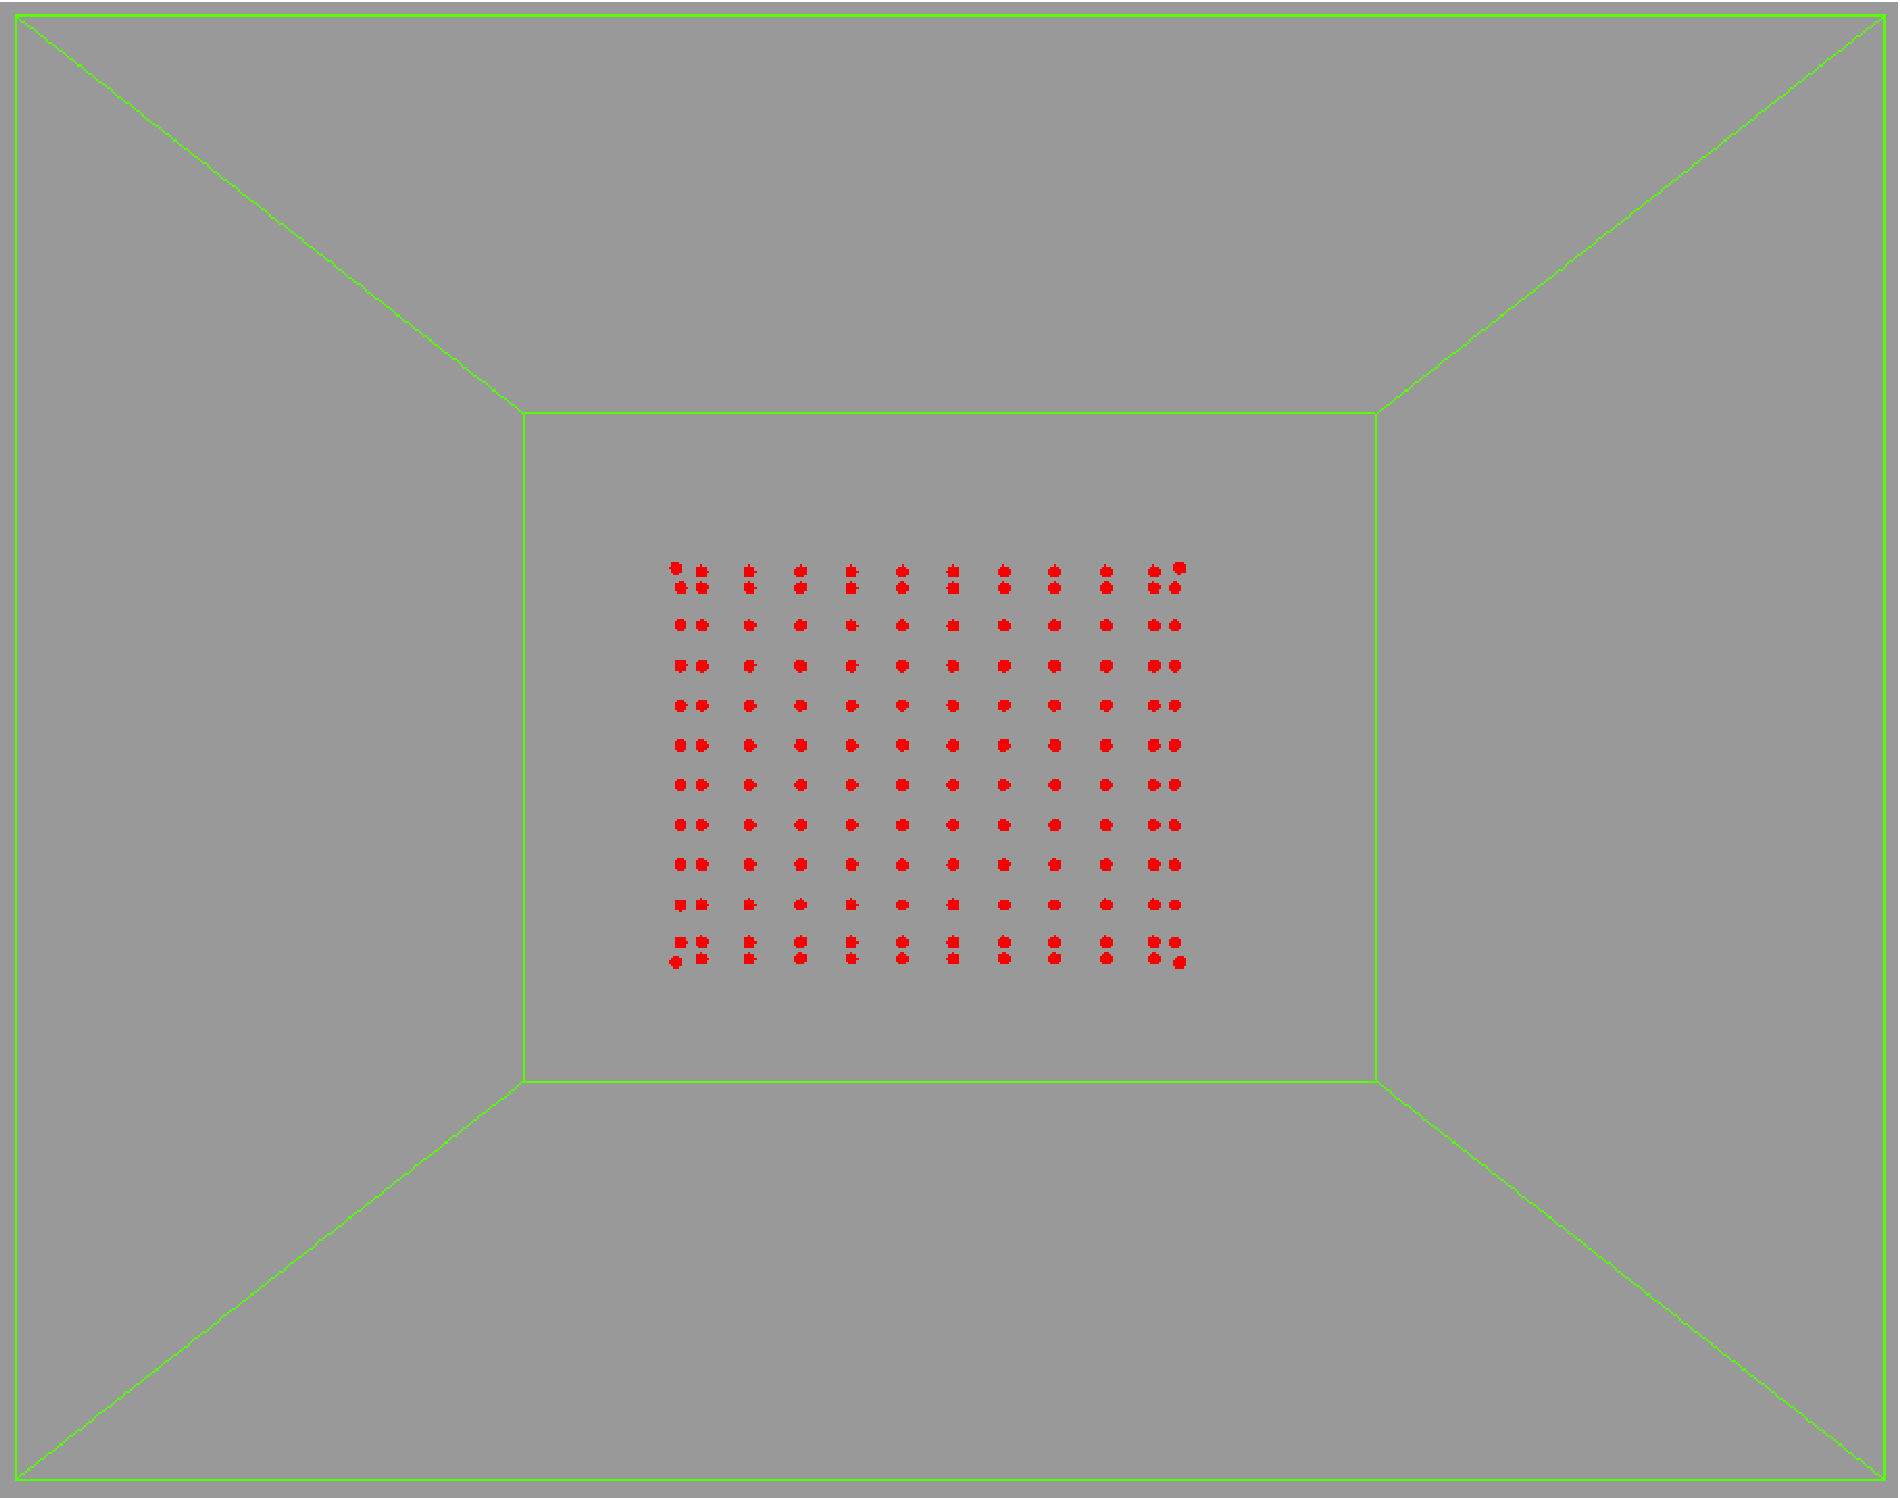
\includegraphics[scale= 0.25]{../figures/coh1.pdf} &
	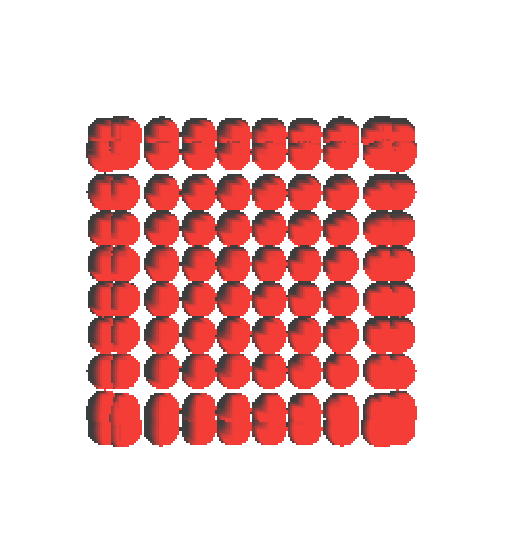
\includegraphics[scale= 0.25]{../figures/coh2.pdf} \\
	
\includegraphics[scale= 0.25]{../figures/coh3.pdf} &
	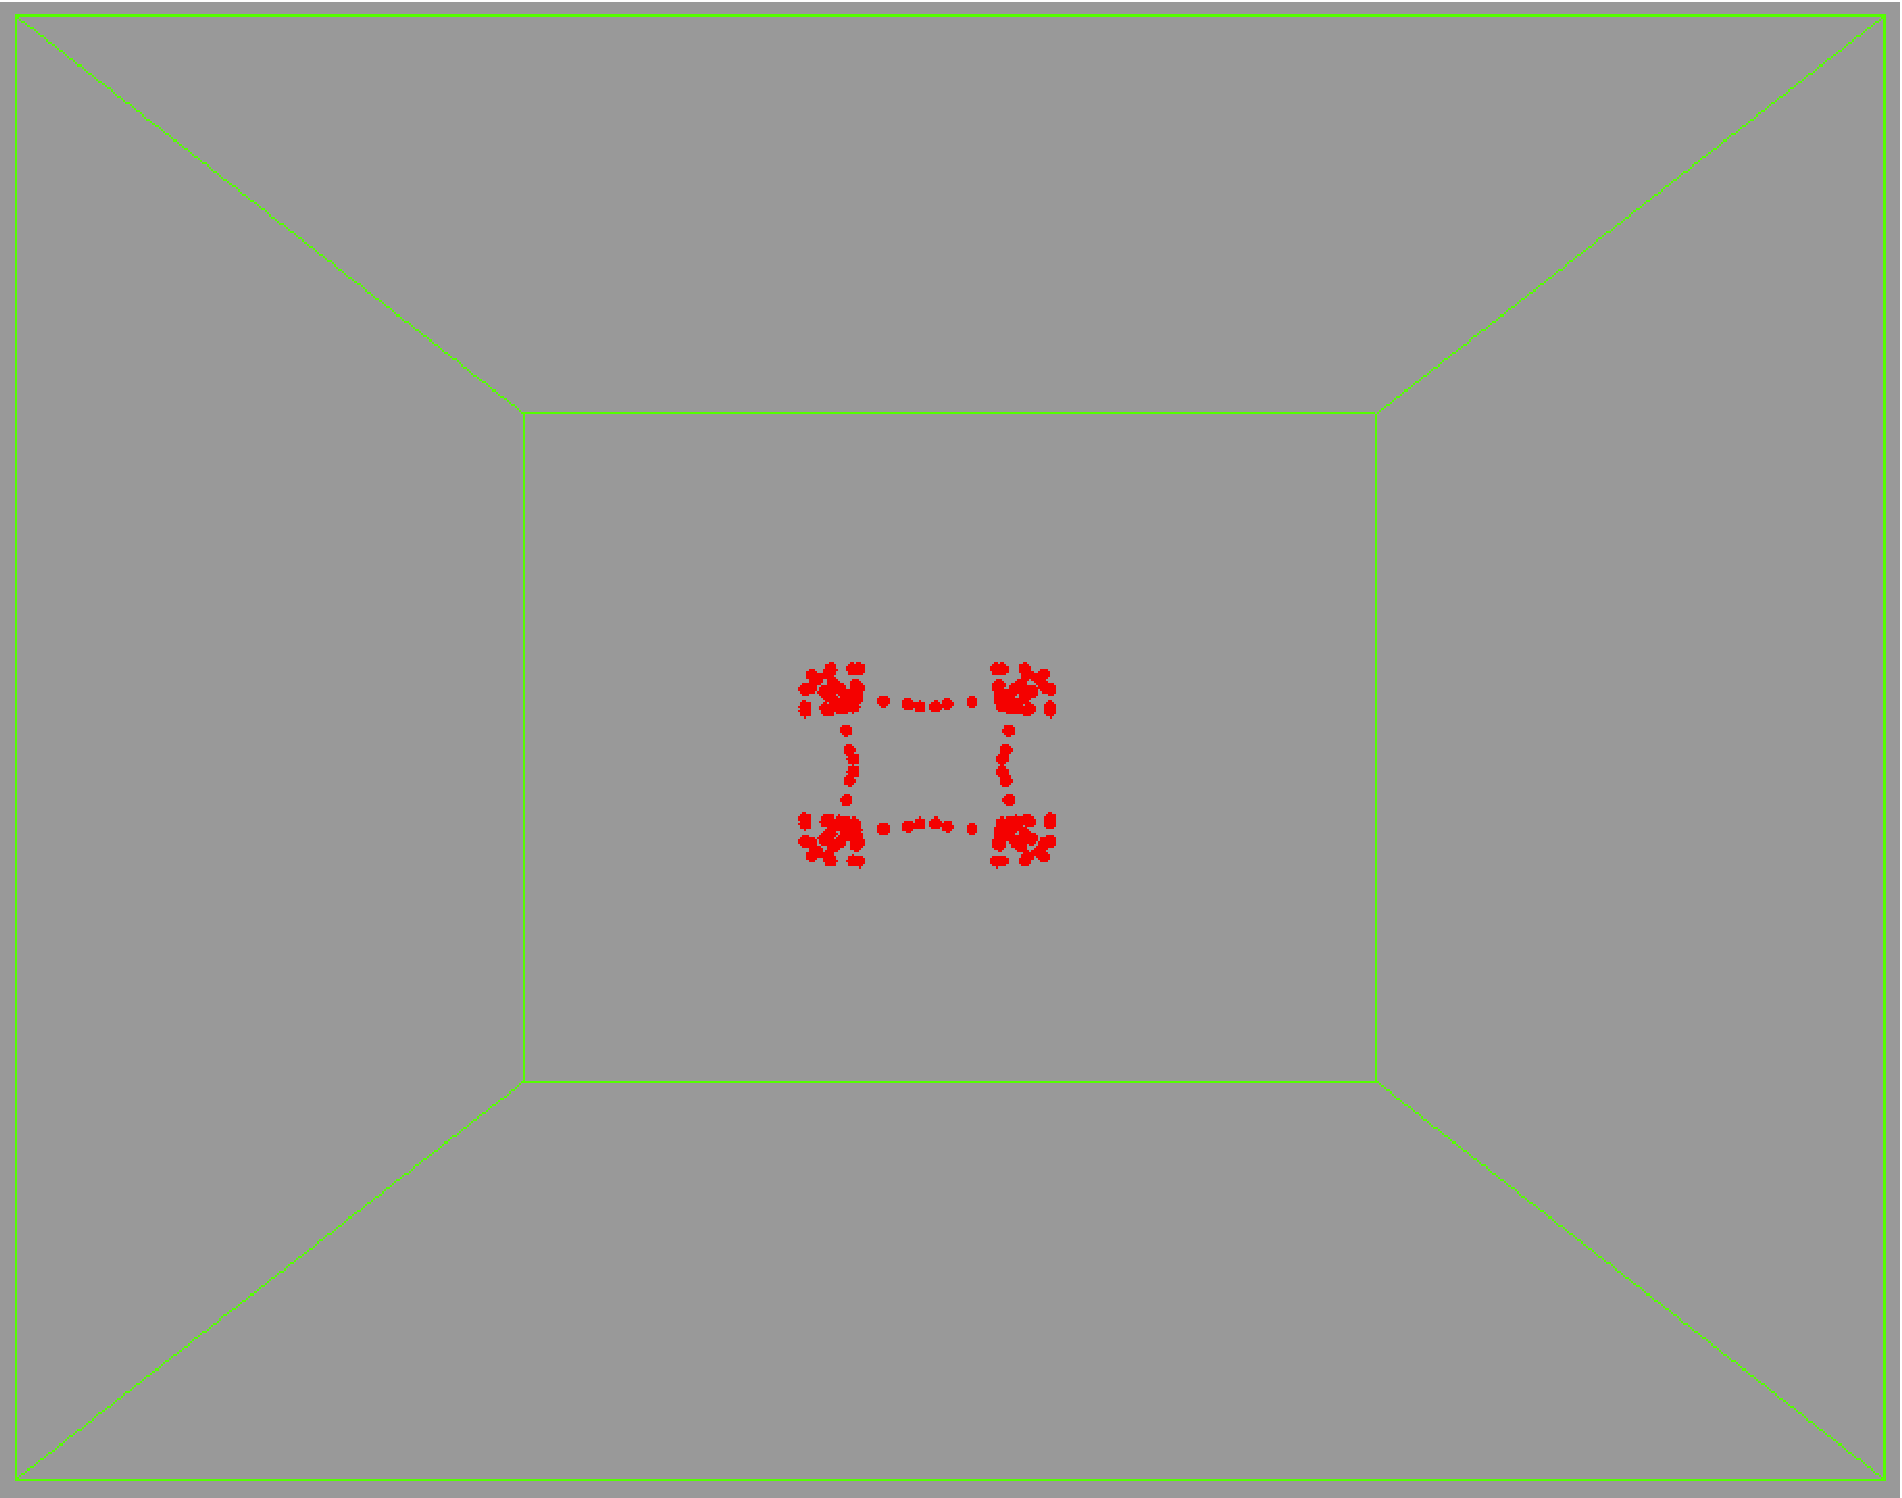
\includegraphics[scale= 0.25]{../figures/coh4.pdf}
	\end{tabular}
	\end{center}
	\caption{Screenshots of the cohesion rule}
	\label{cohRule}
	\end{figure}
\end{frame}

% Blender
\begin{frame}{Blender Demo}
	\begin{figure}[htbp]
	\begin{center}
	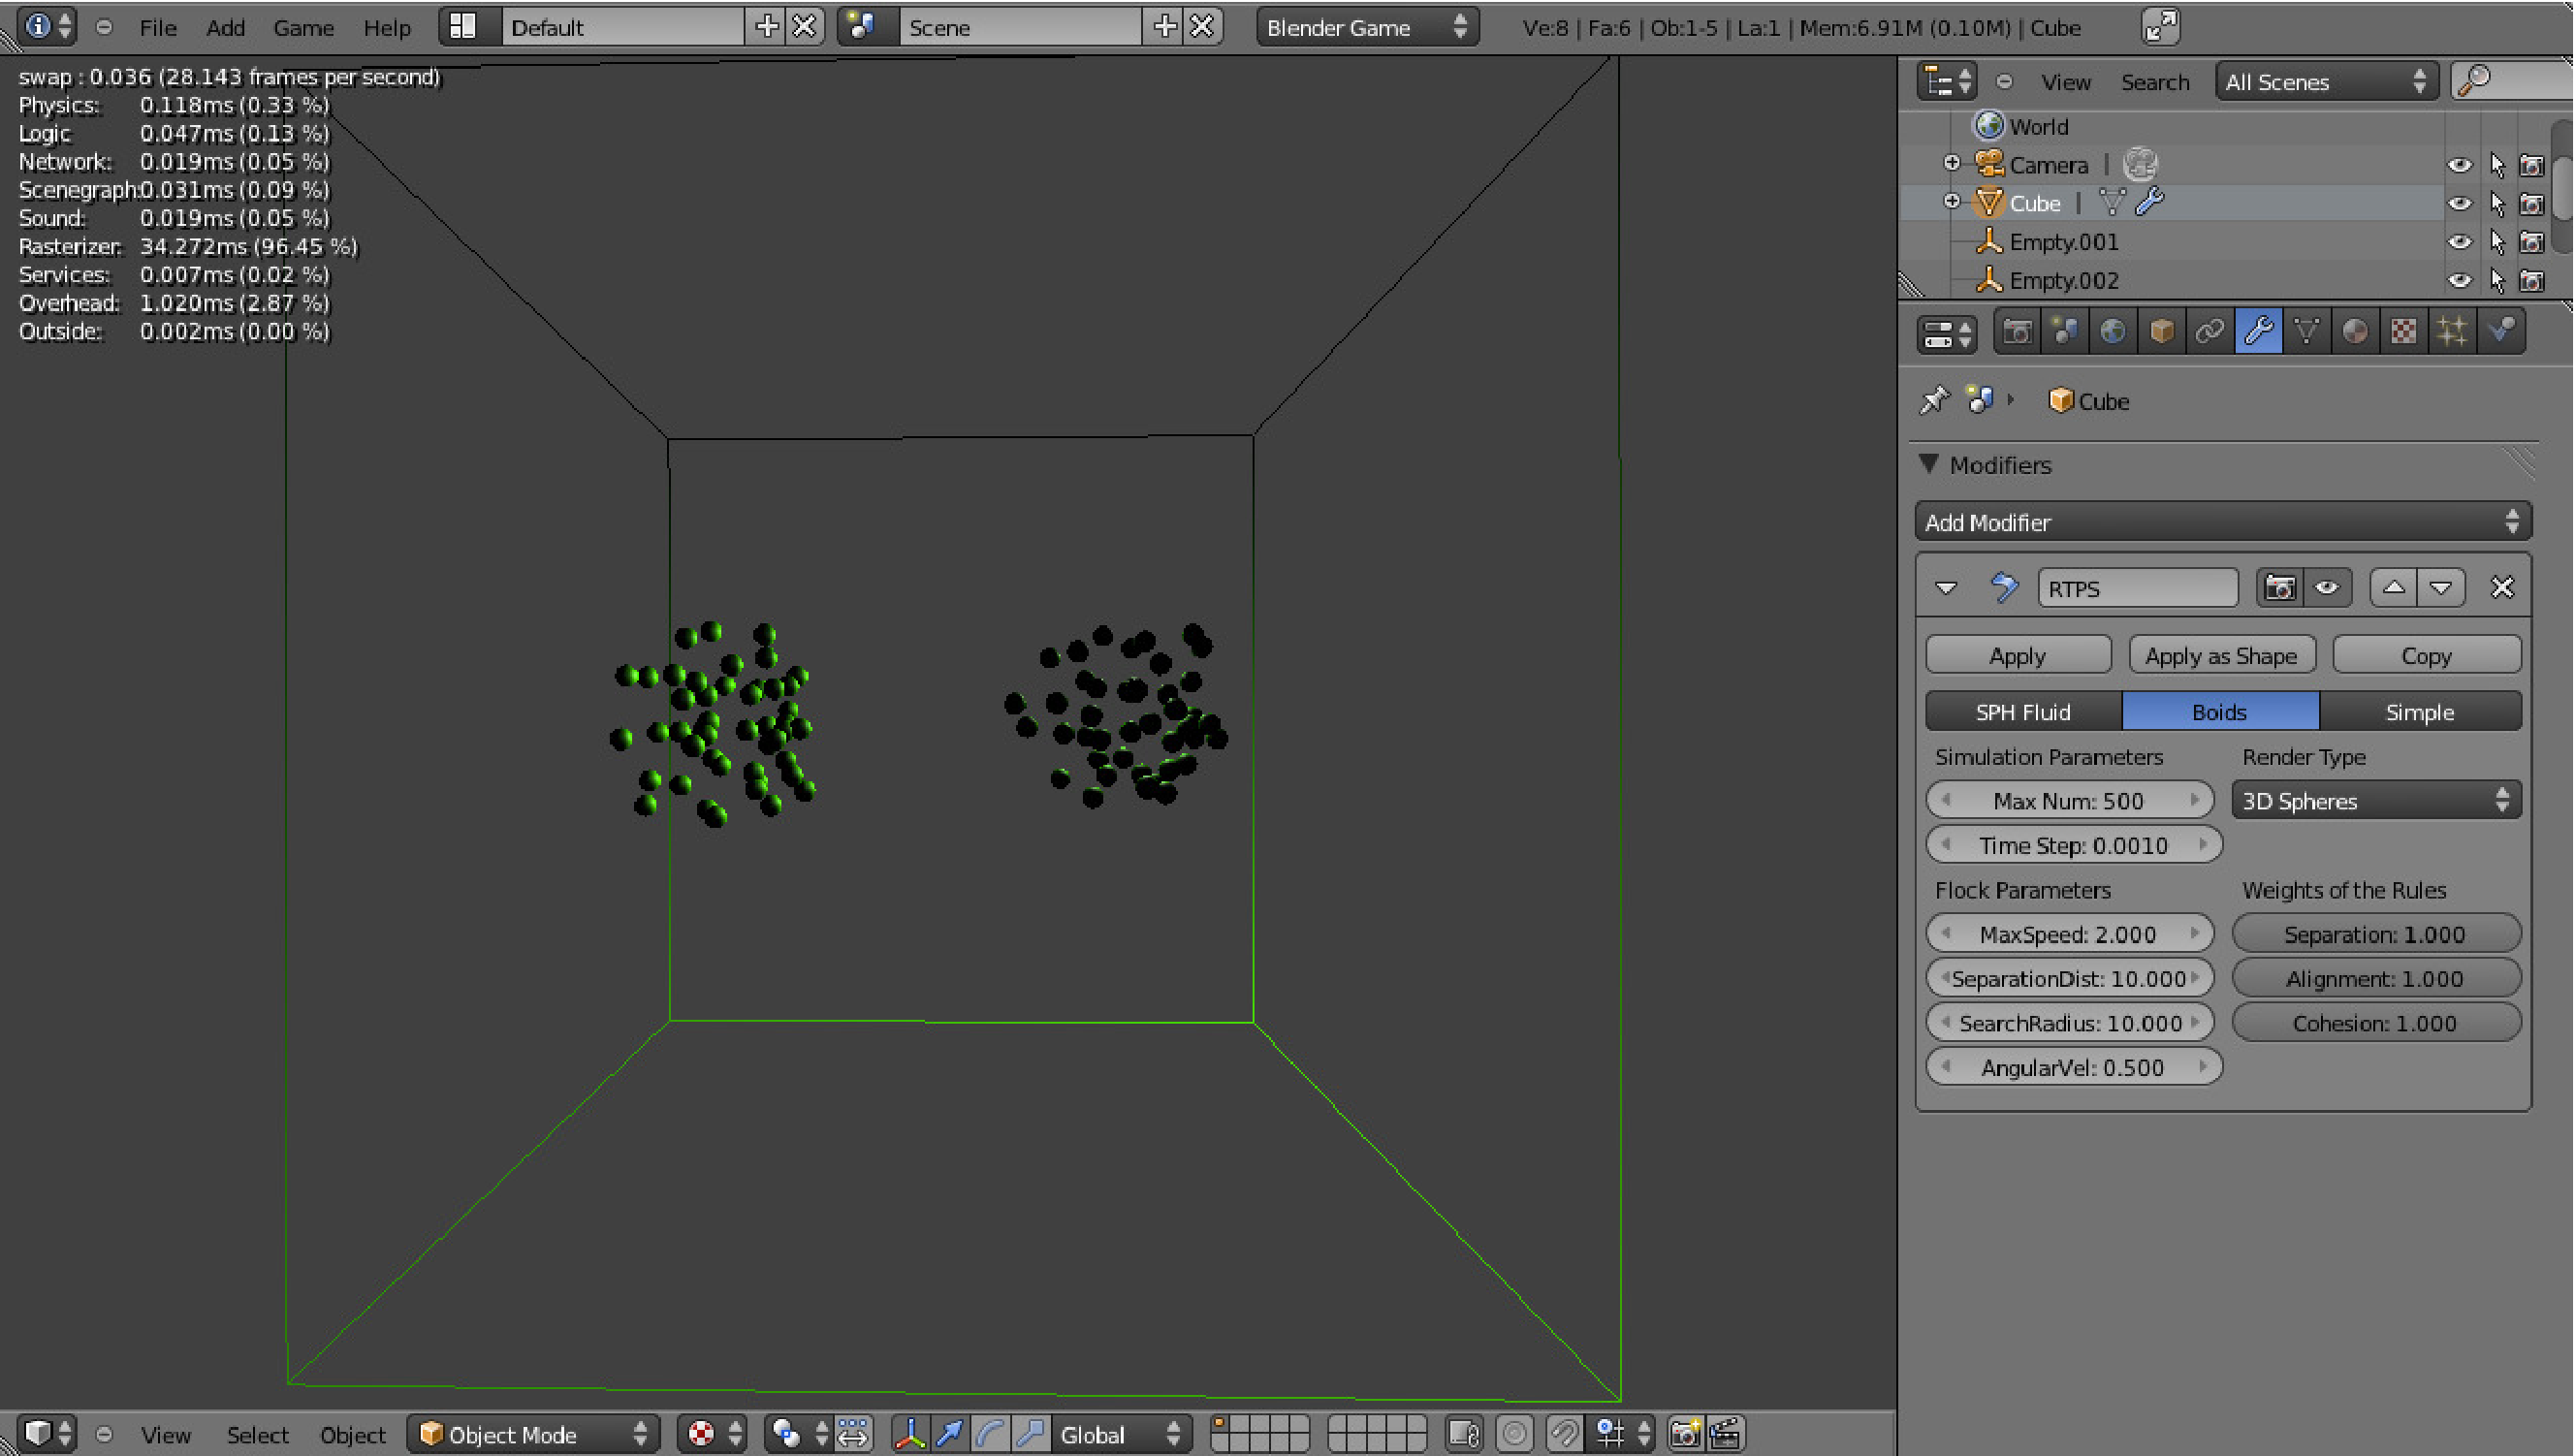
\includegraphics[scale=0.20]{../figures/demo1_1.pdf}
	\caption{Two hoses emitting boids into the FLOCK system}
	\end{center}
\end{figure}
\end{frame}

\begin{frame}{Blender Demo}
	\begin{figure}[htbp]
	\begin{center}
	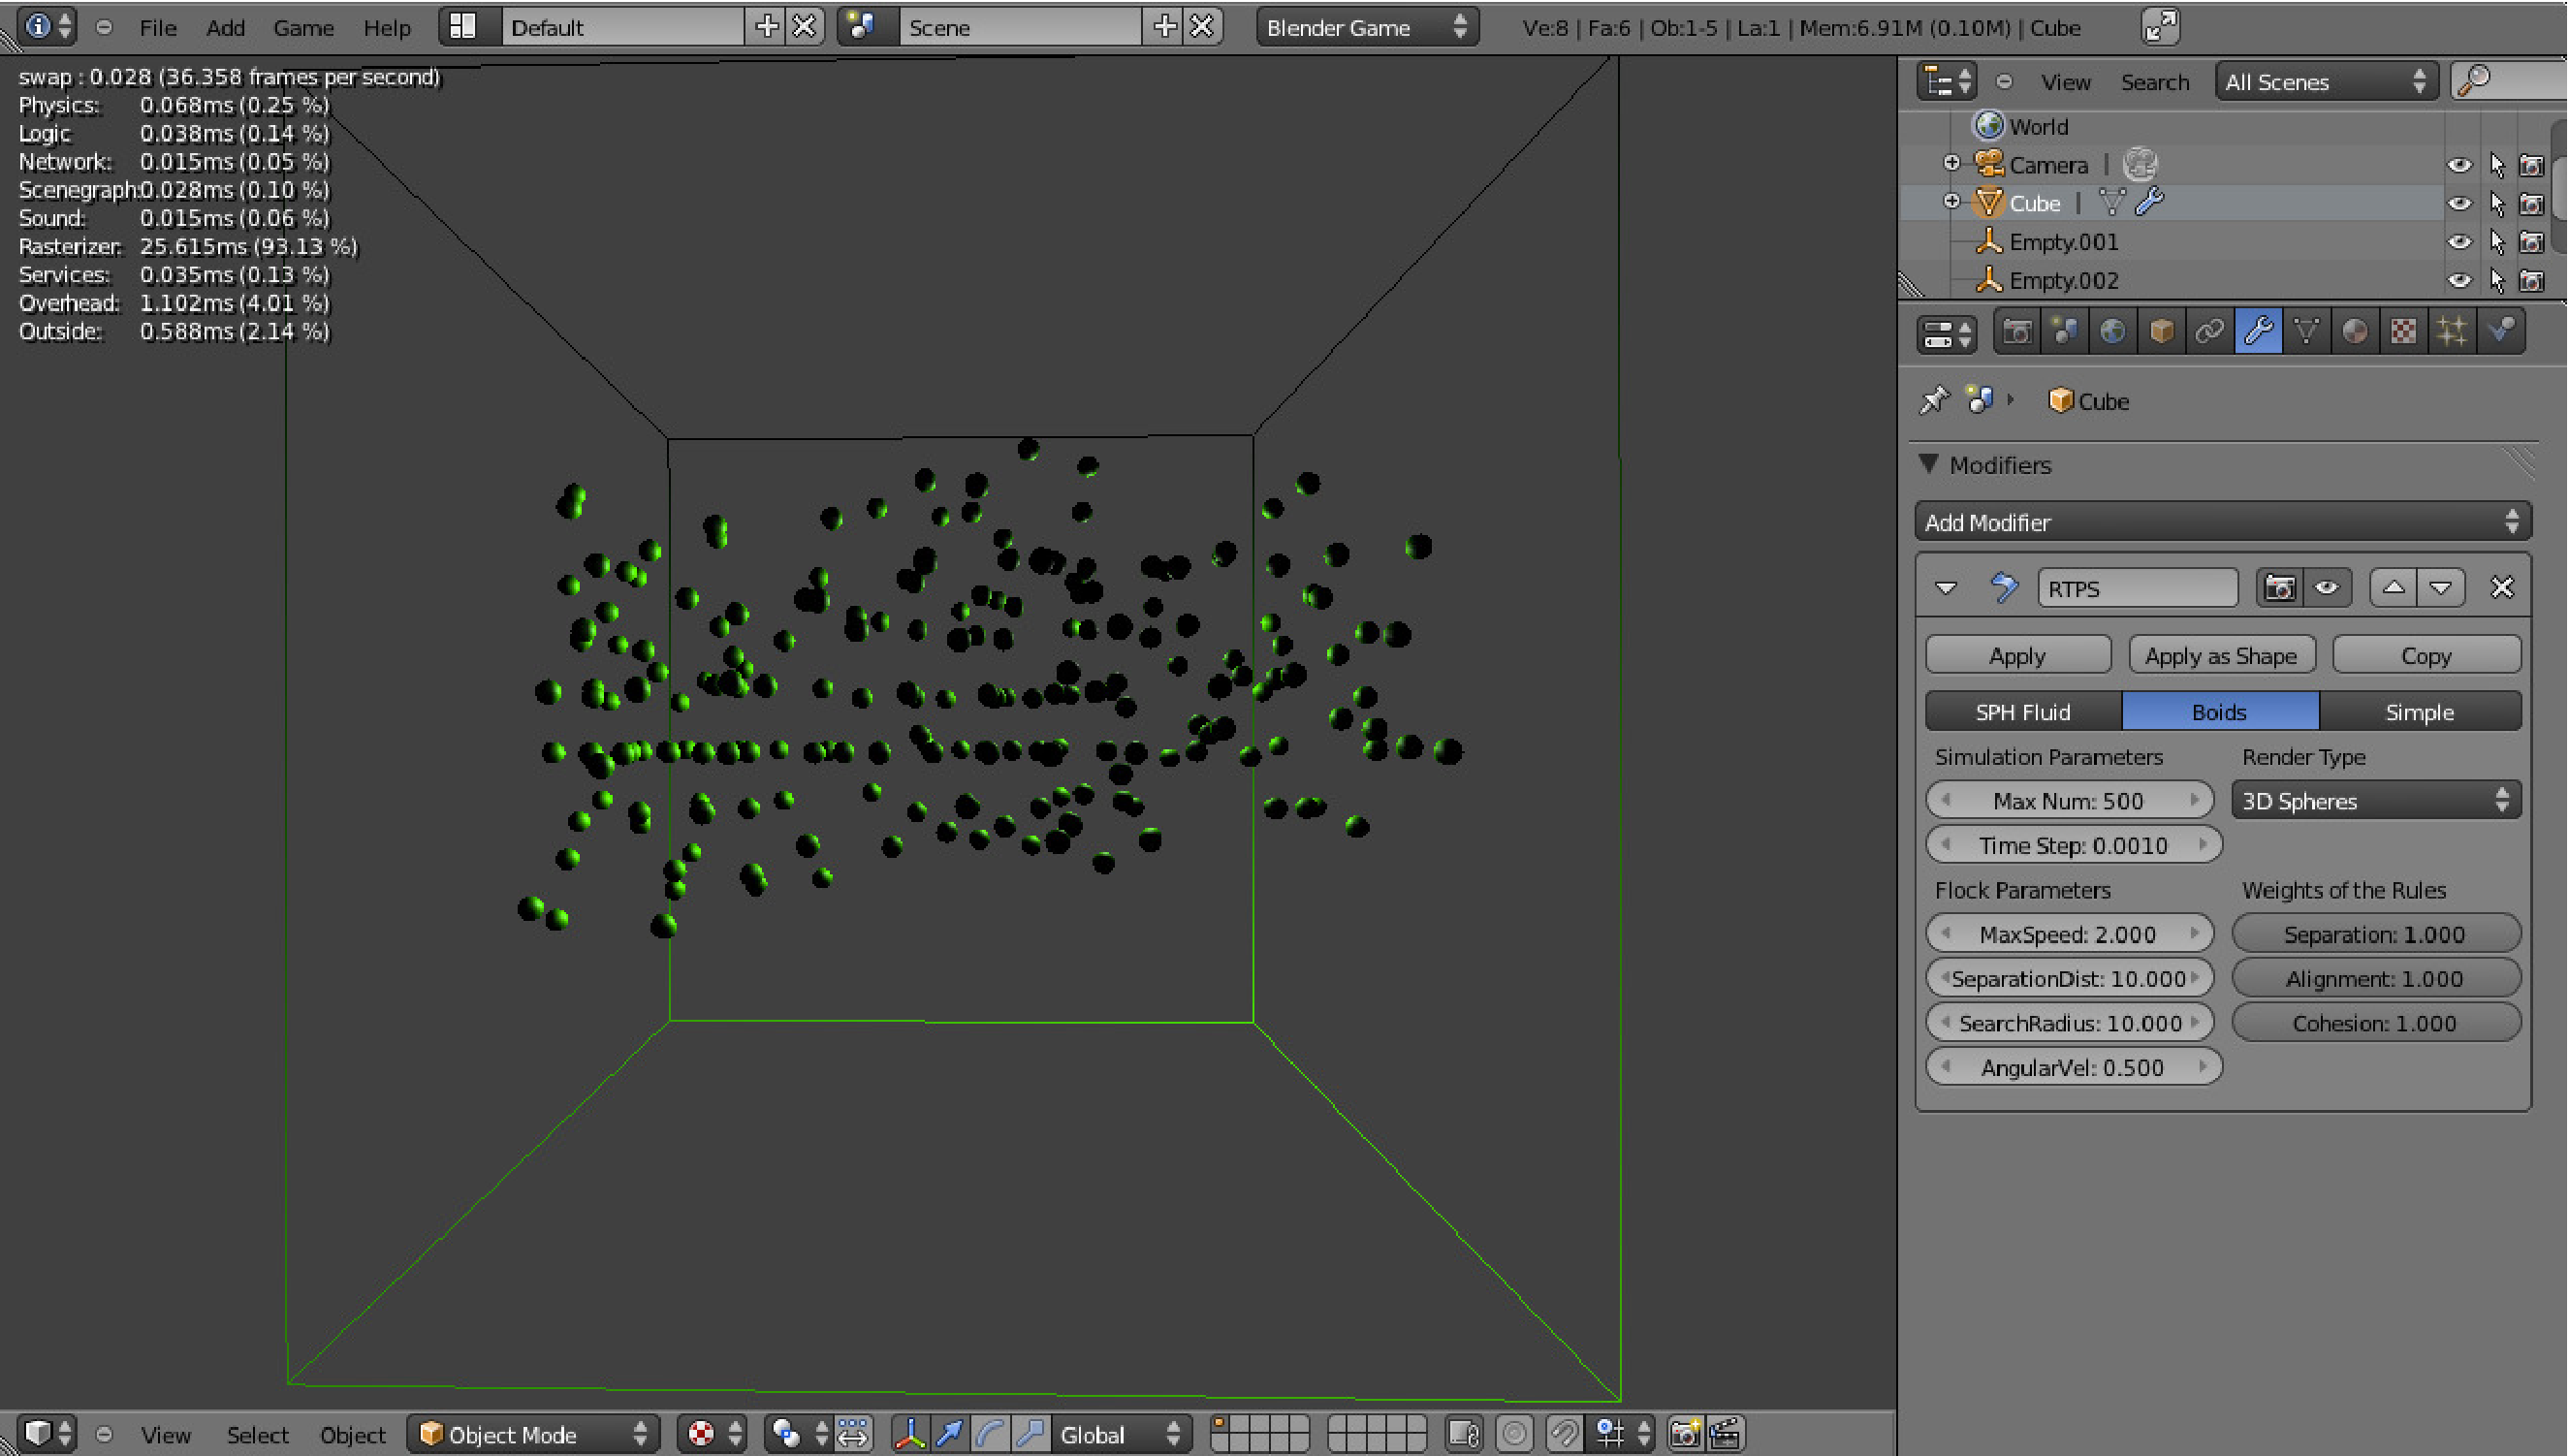
\includegraphics[scale=0.20]{../figures/demo1_2.pdf}
	\caption{Boids are following the rules and they already spread out.}
	\end{center}
	\end{figure}
\end{frame}

\begin{frame}{Blender Demo}
	\begin{figure}[htbp]
	\begin{center}
	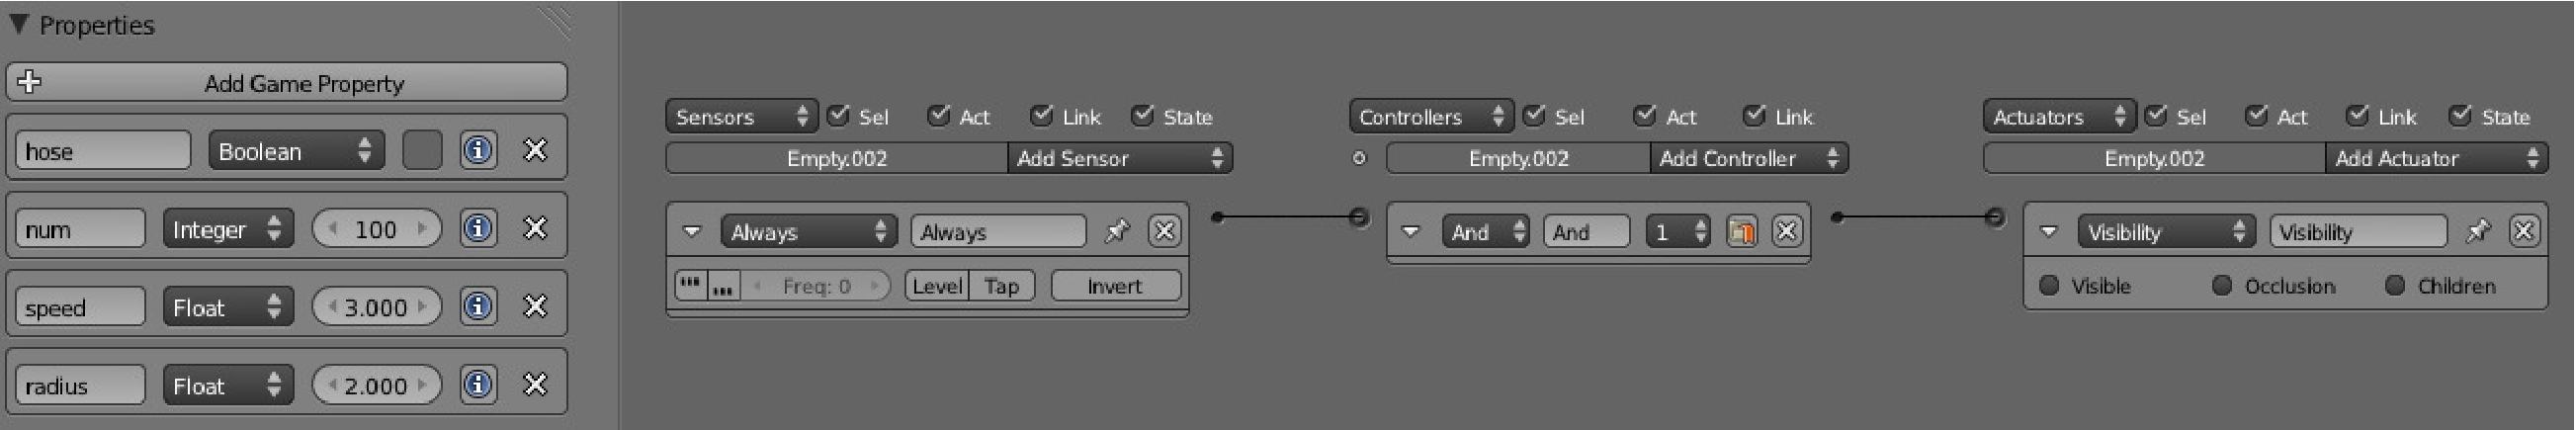
\includegraphics[scale=0.20]{../figures/demo1_logic.pdf}
	\caption{Logic bricks of the first demo.}
	\end{center}
	\end{figure}
\end{frame}


%--------------------------------------------
% conclusion
%--------------------------------------------
\section{Conclusion}
\begin{frame}{Conclusion}
	\begin{itemize}
		\item Using the RTPS library we were able to implement a flocking algorithm in OpenCL.
		\item A custom modifier was developed in Blender to call the RTPS library.
		\item The RTPS modifier able to run a Boids system inside the Blender Game Engine.
		\item The performance of the RTPS modifier outperforms the Boids system of Blender.
	\end{itemize}
\end{frame}

%--------------------------------------------
% future work
%--------------------------------------------
\subsection{Future Work}
\begin{frame}{Future work}
	\begin{itemize}
		\item Expand the list of the implemented rules.
		\item Use Swarm Intelligence or Evolutionary Algorithm to select an optimized set of parameters for the system.
		\item Hybrids systems.
		\item Use Blender objects as emitter particles.
	\end{itemize}
\end{frame}

%--------------------------------------------
%acknowledgments
%--------------------------------------------
\subsection{Acknowledgements}

\begin{frame}{Acknowledgements}
	\begin{table}[htdp]
	\begin{center}
	\begin{tabular}{ccc}
	 & \textbf{Adviser} &\\
	 & Dr. Gordon Erlebacher &\\ 
	& &  \\
	& &  \\ 
	\textbf{Committee} 		&&  \textbf{Special Recognition}\\ 
	Dr. Xiaoqiang Wang 	&&  Ian Johnson\\ 
	Dr. Ming Ye 			&&  Andrew Young\\ 
	 					&&   Evan Bollig \\
	\end{tabular} 
	\end{center}
	\end{table}
\end{frame}

% questions
\begin{frame}
	\begin{center}
	\textbf{Questions?}
	\end{center}
\end{frame}


\end{document}